\documentclass[12pt,oneside,a5paper]{book}

% Paquetes para idioma, tipografía y márgenes
\usepackage[utf8]{inputenc}
\usepackage[spanish,es-nodecimaldot]{babel}
\usepackage{geometry}
\usepackage{graphicx}
\geometry{
    paperwidth=148mm,
    paperheight=210mm,
    top=2.5cm,
    bottom=2.5cm,
    inner=2.0cm,
    outer=2.0cm
}
\usepackage{setspace}
\onehalfspacing

% Paquetes para manejo de colores y páginas de color completo
\usepackage{xcolor}
\usepackage{pagecolor}

% Paquete para eliminar encabezados superiores
\usepackage{fancyhdr}
\pagestyle{plain}

% Configuración de sangría para párrafos
\setlength{\parindent}{1.5em}

% Configuración del Índice: Elimina la numeración (0.1, 0.2, etc.)
\makeatletter
\def\l@section#1#2{\@dottedtocline{1}{0em}{0em}{#1}{#2}}
\makeatother

% Comando para páginas en blanco destinadas a imágenes
\newcommand{\paginaenblanco}{
    \clearpage
    \thispagestyle{empty}
    \null
    \clearpage
}

% Comando para portadas de capítulos en NEGRO con texto EN BLANCO y línea delgada
\newcommand{\capituloconportada}[1]{
    \clearpage
    \newpagecolor{black}
    \color{white}
    \thispagestyle{empty}
    \vspace*{\fill}
    \begin{center}
        {\Huge \bfseries \MakeUppercase{#1}} \par \vspace{0.6em}
        {\color{white}\rule{0.6\textwidth}{0.4pt}}
    \end{center}
    \vspace*{\fill}
    \clearpage
    \restorepagecolor
    \color{black}
    \addcontentsline{toc}{chapter}{#1}
}

% Comando personalizado para cada poema: abre en página propia con línea delgada debajo del título
\newcommand{\poema}[1]{
    \clearpage
    \section*{#1}
    \vspace{-0.5em}
    {\color{black}\rule{\textwidth}{0.4pt}} \par \vspace{0.8em}
    \addcontentsline{toc}{section}{#1}
}

\begin{document}

% ---------------------------------------------------------
% PORTADA (Fondo Negro - Texto Blanco con línea decorativa)
% ---------------------------------------------------------
\begin{titlepage}
    \newpagecolor{black}
    \color{white}
    \centering
    \vspace*{\fill}
    {\Huge \bfseries Muerte del letargo \par}
    \vspace{0.5em}
    {\color{white}\rule{0.7\textwidth}{0.4pt}} \par
    \vspace{2cm}
    {\Large Maldonado Jose \par}
    \vspace*{\fill}
\end{titlepage}
\restorepagecolor
\color{black}

% ---------------------------------------------------------
% ÍNDICE GENERAL
% ---------------------------------------------------------
\clearpage
\tableofcontents
\clearpage

% ---------------------------------------------------------
% PRÓLOGO
% ---------------------------------------------------------
\chapter*{Prólogo}
\vspace{-0.5em}
{\color{black}\rule{\textwidth}{0.4pt}} \par \vspace{0.8em}
\addcontentsline{toc}{chapter}{Prólogo}

Muerte del Letargo es la primera obra de José Efraín Maldonado Rangel, un joven escritor venezolano radicado en Argentina, escrita durante un período de transformación personal, sentimental y emocional. La obra nace de la necesidad de romper con aquello que nos mantiene inmóviles y de encontrar, incluso en medio del caos, una forma de avanzar.

El poemario se divide en tres partes: Caos, Zen y Éter. Cada una representa un momento distinto del proceso: la confrontación, la búsqueda de equilibrio y aquello que permanece después de haber atravesado la turbulencia.

Los poemas recorren la pérdida, el deseo, la soledad, el amor, la incertidumbre y la necesidad de liberarse de aquello que alguna vez pareció imposible abandonar. El lenguaje también se abre a otras culturas mediante palabras extranjeras que permiten nombrar sentimientos para los que, a veces, nuestra propia lengua parece insuficiente.

Muerte del Letargo no pretende contar una historia lineal ni ofrecer una superación perfecta. Es el registro de un despertar: el momento en que permanecer inmóvil deja de ser una opción.

“La vida es demasiado corta para lamentarse; levántate y busca tu emancipación.”

% ---------------------------------------------------------
% CAPÍTULO 1: CAOS
% ---------------------------------------------------------
\capituloconportada{CAOS}

\poema{Perdida}
La paciencia no es uno de mis fuertes; por lo general, quiero todo lo más rápido posible para no correr el riesgo de perderlo.

¿Se puede perder algo que nunca fue tuyo?

Me perdí a mí mismo mientras buscaba a alguien. Lo encontré; sin embargo, terminó siendo un destello fugaz que se llevó consigo una parte de mí que otros desertores también querían.

“… Y dijo Jesús a sus apóstoles: Tomad y comed todos de él, porque este es mi cuerpo, que por vosotros es partido; haced esto en conmemoración mía…”

Intenté ser un salvador para las almas dolidas, entregando partes de mí que fueron dejando espacios en blanco que aún me cuesta llenar.

Creo ser bueno e intento siempre serlo. Digo no esperar nada a cambio, mientras conservo la esperanza de recibir algún día un poco del amor que doy.


\poema{Negación}
Tuve la llave siempre frente a mí, pero caminé en sentido contrario, ignorando la voz interna que me pedía no huir.

Una y otra vez elegí saltar por la ventana cuando la puerta de oro estaba justo allí, esperando.

Rompí vidrios, arranqué cortinas, destruí personas y cosas, buscando la luz que atravesaba el vitral de aquella catedral donde solía perderme por las tardes.

Entonces, no me creía digno de nada más que del silencio: ciego, entregado al abismo de mi propio castigo.

¡Ayuda!

Nada de esto se repite. Todo es nuevo…

Y estoy aterrado.


\poema{Ira}
Arranqué cada sonrisa del álbum fotográfico. Ebrio de dolor, mi única compañía: una copa de vino medio vacía y un bolígrafo moribundo que apenas susurraba letras.

Sentía el gemido de la cuartilla bajo la presión de mis palabras, como si cada frase fuera un vómito de mi alma intoxicada.

Las lágrimas caían, catarata sin destino, y al tocar la tinta la volvían confusa, como yo, que también había perdido el rumbo.


\poema{Apatía}
El egoísmo puede doler como un filo hundido en el pecho. Decir palabras vacías por un instante de falsa felicidad hiere incluso al alma más marchita.

Él notaba mi silencio; la incomodidad lo rozaba como a un culpable atrapado en su reflejo. Preguntaba con falsa sorpresa:

—¿Qué pasa? 

—¿Por qué tan callado? 

—¿Ahora por qué lloras?

No… no se dio cuenta. Y tal vez eso fue lo peor.
Me hirió y luego actuó como si nada, como si mi dolor no tuviera nombre.

Cada silencio era una hojilla afilada, cortando lentamente el hilo rojo que nos unía a la nada.


\poema{Vacío}
En el interior de la caja fuerte, una copa del cristal más delicado reposa; si quieres, puedes beber de su dulce contenido.

El péndulo del reloj va y viene. ¡Corre!, te está alcanzando. Suelta todo lo que llevas sobre ti; al final, nada traes y nada te llevas. Toma las manos que te ofrecen para impulsarte, pero no te encariñes con todas; solo unas pocas te instigarán a volar.

Mientras más avanzas, más se fisura tu copa; por mucho que resista la caja, hay manos infames que logran tocar la delicada pieza.

Maldición, está rota.

Recoges cada pequeño cristal, aunque se claven en lo más profundo de tu piel, provocándote heridas.

Te torturas una y otra vez sin darte cuenta de que la copa era reemplazable.

Las heridas de tus manos, no.


\poema{Certidumbre}
En el conticinio de la noche, los gemelos nadan en medio de la lid; dos titanes danzan frente a frente, magníficos, casi celestiales.

¿Quién ganará?

¿El ángel o el demonio?

Los observo luchar como quien contempla su propio destino sin atreverse a intervenir.

Hasta que ocurre.

Ruptura.

Mi boca se mancha. Intento hablar, pero la mancha crece, se extiende con cada palabra, con cada plegaria que mi alma grita en silencio.

Ya no sé si quiero hablar o simplemente sangrar.
La mancha lo cubre todo hasta convertirse en dolor: un dolor extraño, casi hermoso, porque tiene la certeza de una batalla terminada.

Y entonces comprendo:

gané.

El ángel venció al demonio, o quizá fue al revés.

Ya no importa.

Porque mientras celebraba la victoria, algo dentro de mí también cayó.

Gané la batalla,

pero perdí una parte de mí.

\clearpage
\thispagestyle{empty}
\begin{figure}[h!]
    \centering
    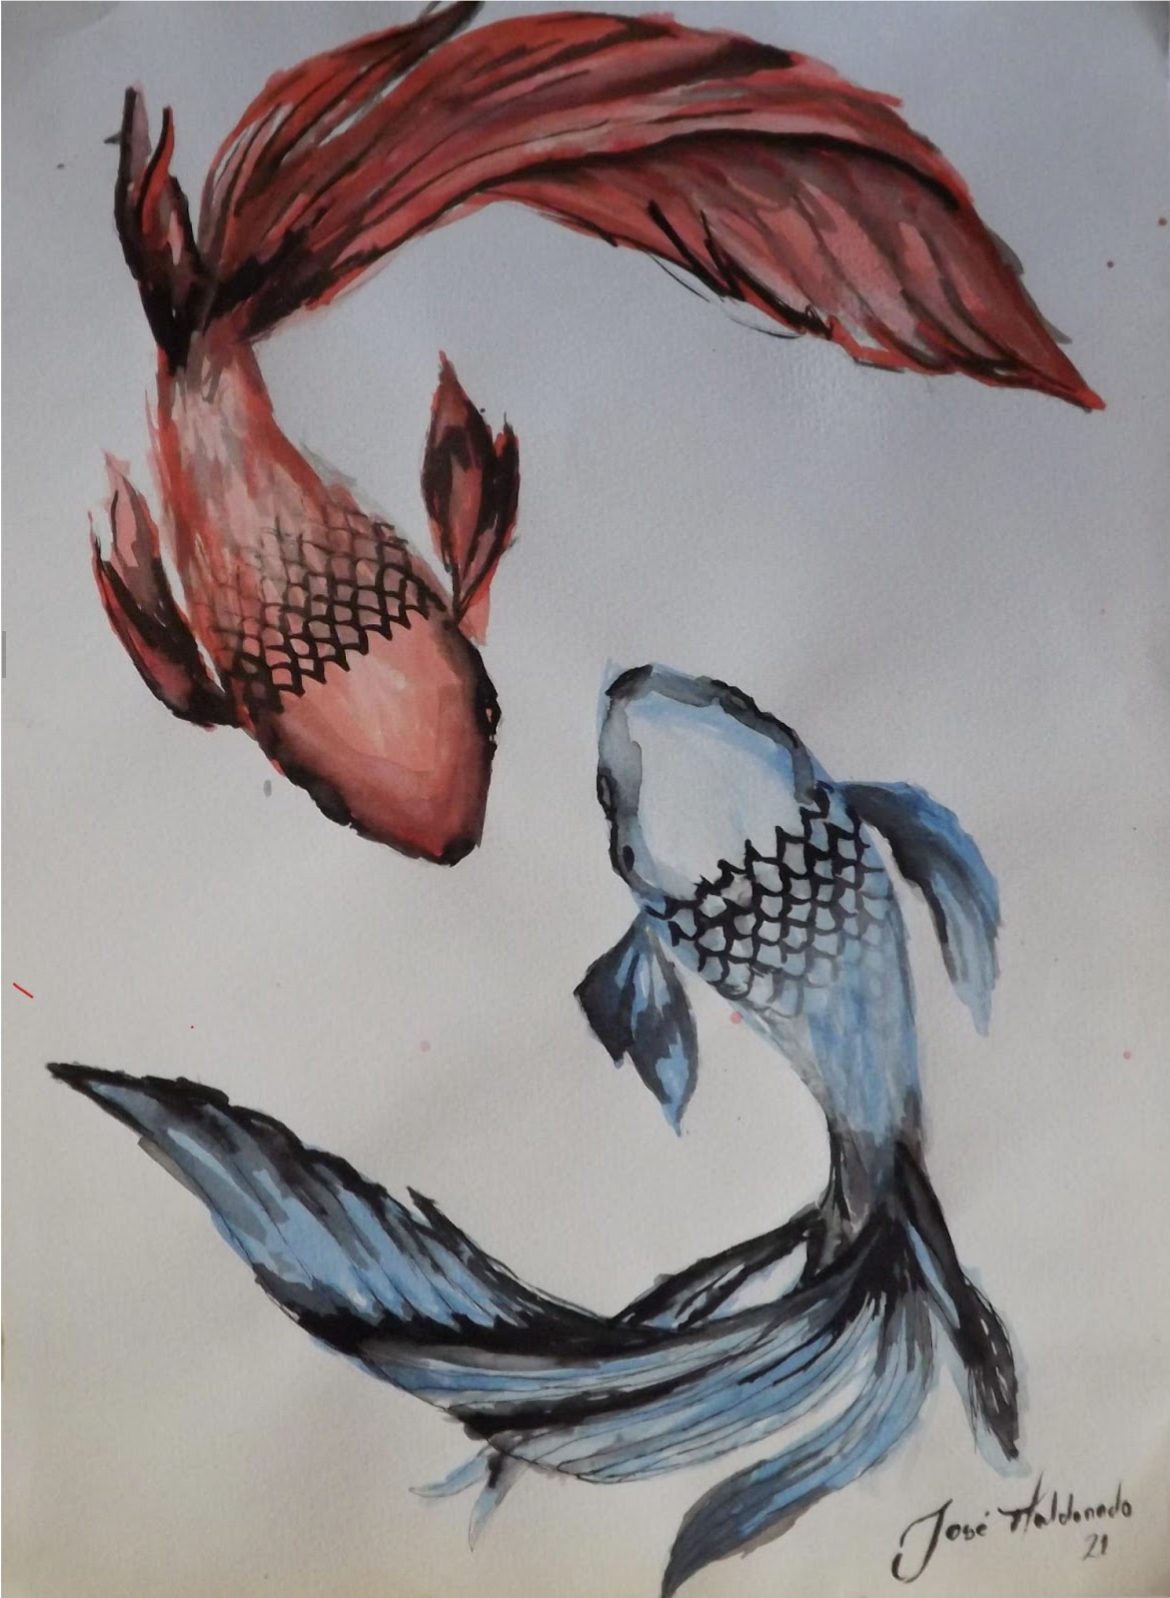
\includegraphics[width=1.0\textwidth]{certidumbre.png}
\end{figure}
\clearpage

\poema{Traspié}
La vida sin drama es como una comedia sin risas; una existencia sin rumbo, floreciendo hacia ninguna parte.

Caminaba descalzo por la nieve, en una noche tormentosa revestida de perla y azul. Cada paso dolía, pero mi intuición, raramente equivocada, seguía guiándome.

Entonces lo vi.

Un faro, con una luz tenue pero cálida, brillaba en medio del estruendoso desastre.

Llegué hasta él y me cobijé bajo su resplandor. A la distancia brillaban otros más, pero aquella luz tenía todo lo que necesitaba.

No era la más grande. 

Ni la más intensa.

Era simplemente la que encontré cuando más perdido estaba.

Y quizá eso bastaba.

Porque después de tanto caminar sin saber hacia dónde, comprendí que no siempre hay que encontrar el camino.

A veces solo hace falta una luz que nos convenza de dar el siguiente paso.

Robaré el brillo de una estrella fugaz para guardarlo conmigo, para que la promesa del mañana no se esfume.


\poema{Cara o sello}
Como un animal entre las sombras, la quimera espera agazapada; solo una moneda decidirá cuál de sus caras encontrarás.

Una cara sabe de compasión, de amor, comprensión y entrega. La otra difiere de lo bueno: conoce el miedo, el rencor y la ira.

Una te abrirá los brazos. La otra esperará el momento menos pensado para saltar y cortar tu cuello.

Pero ambas son la misma criatura.

Ese es su peligro.

La quimera tiene una debilidad: se encariña con cualquiera que intente dominarla.

Y aunque sabe que terminará herida, persiste.

Se entrega. 

Perdona. 

Vuelve.

Hasta que la hieren una vez más.

Te lo advierto:

no te dejes engañar por la cara que te sonría.
Aunque creas que es tuyo, aunque creas haberlo domesticado, en el momento en que lo hieras descubrirás la verdad:

no era un sueño ideal.

Era una pesadilla aprendiendo a quererte.


\poema{Libertad}
Las casualidades y las coincidencias no existen, aunque a veces en silencio persisten. Un teatro vio nacer, sin previo aviso, el fervor de dos amantes que el destino quiso: uno venezolano, otro argentino, dos desconocidos cruzándose en el mismo camino.

Temerosos y emocionados, se encontraron sin saber qué les esperaba a ambos lados. Bastaron unas sonrisas, sencillas y sinceras, para hacer de unas horas una historia verdadera.

Una regla de oro, fundamental, se rompió aquella noche de manera accidental, por aquel bohemio extranjero que solo buscaba hacer sonreír al triste aventurero.

Después llegaron noches de pasión, dos amantes separados, unidos por la imaginación. Solo con sus pensamientos hicieron el amor, como si el deseo pudiera vencer al temor.

Fueron pocos los días que el destino les concedió, pero bastaron para saber que algo entre ellos nació. Juntos rompieron estigmas, miedos y cadenas, descubriendo que algunas prohibiciones no valen la pena.

Y llegó la última noche, inevitable despedida, una cena con un hermoso toque recorriendo la ciudad dormida. Todo parecía conducir hacia el broche final, como si Buenos Aires quisiera guardar aquel ritual.

El Teatro Colón los vio juntar. El Teatro Colón los vio separar.

Y así terminó aquel encuentro inesperado: uno siguió su camino, el otro quedó con el recuerdo guardado.

Un amante de invierno voló hasta mi vida… espero verlo algún día.

\clearpage
\thispagestyle{empty}
\begin{figure}[h!]
    \centering
    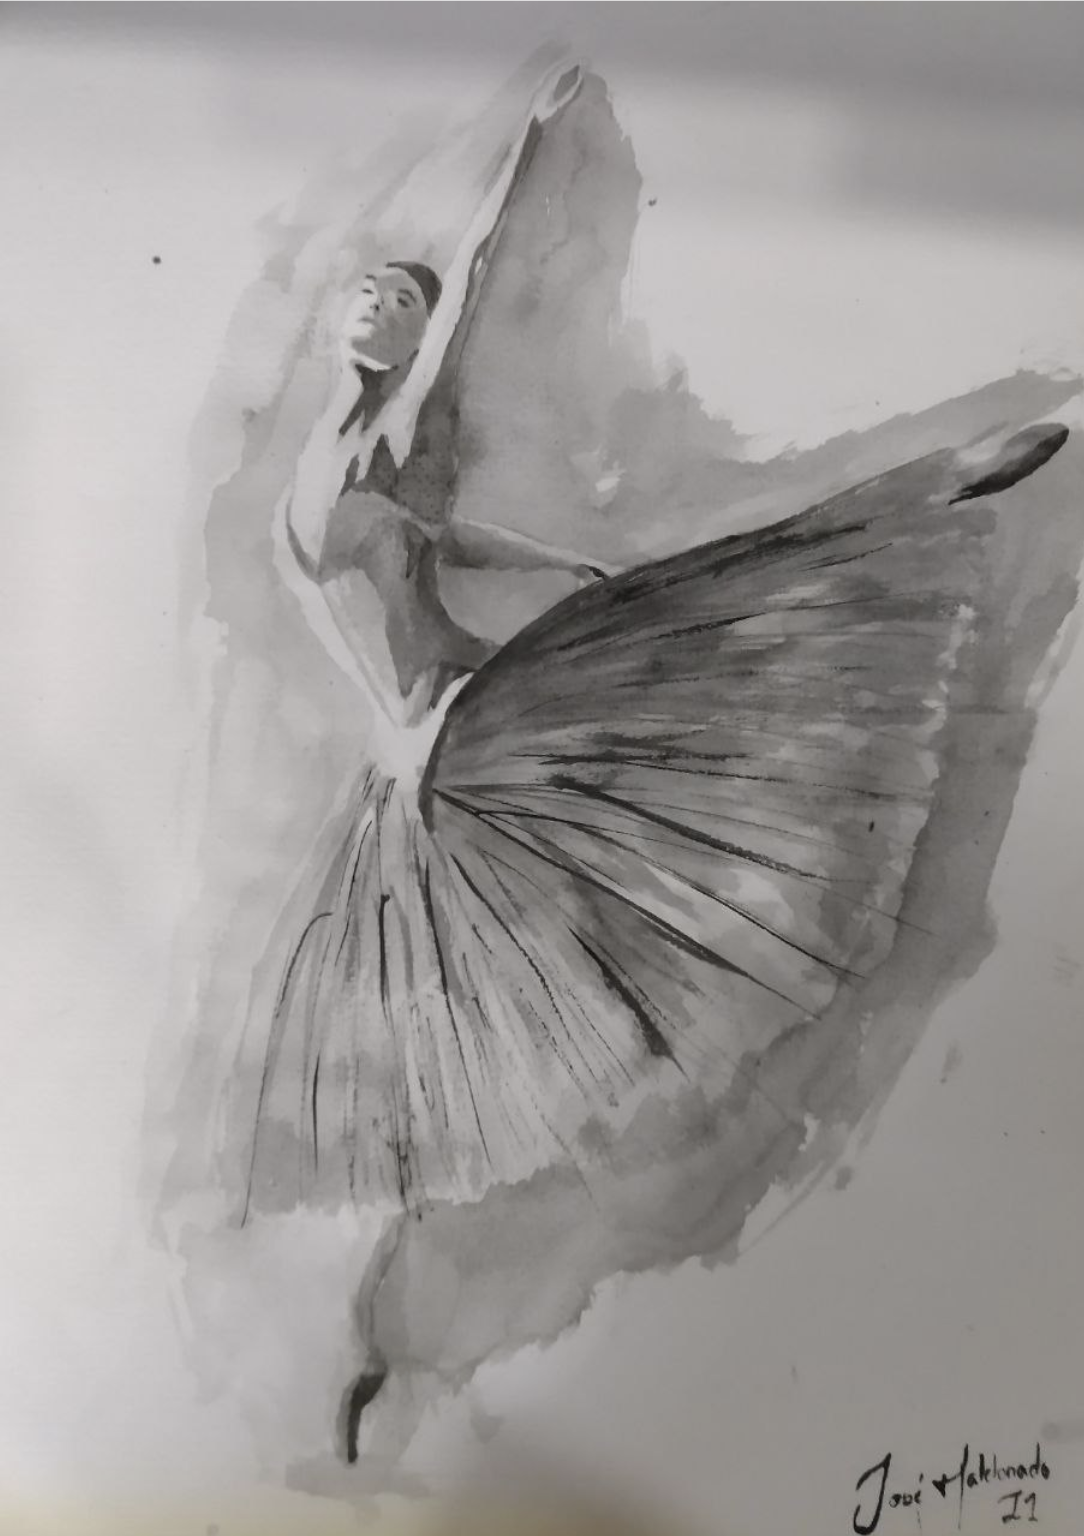
\includegraphics[width=1.0\textwidth]{libertad.png}
\end{figure}
\clearpage


\poema{Olvido}
Somos hijos del tiempo, propensos a convertirnos en una eternidad o en un santiamén durante el largo camino de la vida.

Líneas que nadan contra la corriente y otras que avanzan a su favor, destinadas a encontrarse en algún punto, combinarse y ser una sola, o simplemente acompañarse durante un breve instante en la espesa y vasta nada del infinito.

Seres destructivos que marcamos un principio, pero no un fin.

Tantas huellas impresas en la piel que desaparecen en un abrir y cerrar de ojos; tan pocas huellas parchadas en el alma que ni la misma muerte conseguirá borrarlas.

Cada uno decide qué quiere ser:

un fragmento del complejo rompecabezas,
o el rompecabezas en su máxima expresión.


\poema{Bangover}
Mis palabras son como un manantial de poemarios que quieres beber.

Te acercas lo suficiente para no darte cuenta de que ya estás dentro.

Y una vez que bebes de mí, ya no puedes salir.
Soy la prosa que escucha tu oído, el verso que acalora tus sentidos; soy aquello que quieres poseer, pero que jamás te va a pertenecer.

Quieres arrebatarme, pero me deslizo entre tus dedos, dejando apenas un rastro húmedo de mí que, con el tiempo, se evaporará, exaltando tu melindrosa codicia y tu avaro apetito.

Por más que quieras dejarlo, no podrás.

Porque en este juego las reglas las pongo yo.

Puedo quedarme, puedo seguir jugando, puedo dejarte beber de mí hasta saciar tu deseo.

Pero si decido marcharme, todo lo que quieras dejará de importar.

Porque al final, no eres tú quien decide cuándo termina el juego.


\clearpage
\thispagestyle{empty}
\begin{figure}[h!]
    \centering
    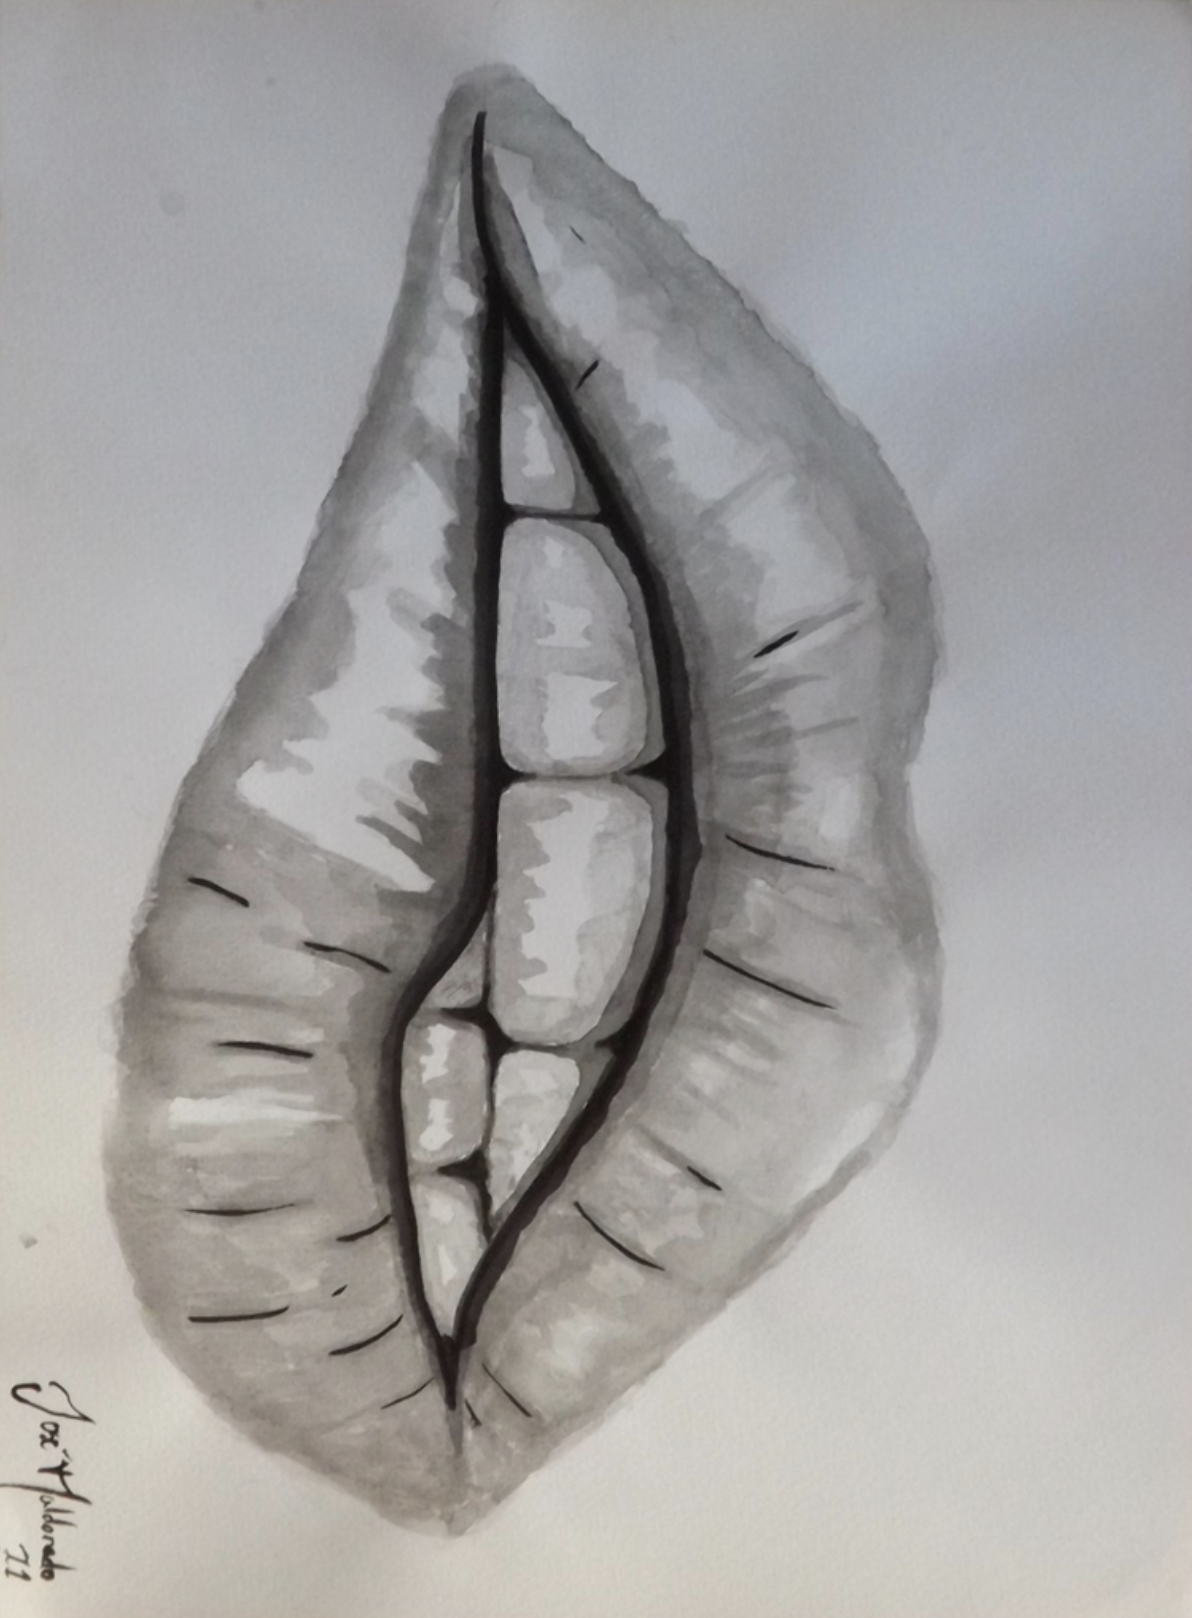
\includegraphics[width=1.0\textwidth]{bangover.png}
\end{figure}
\clearpage

\poema{Verano en invierno}
Dos personas de distinto proceder, destinadas a encontrarse al atardecer. Uno, de carácter decidido y tenaz; el otro, sereno, tranquilo y sagaz.

La vida los había recorrido sin piedad, dejando cicatrices bajo una misma verdad. Uno aprendió a esconderse detrás del dolor, mientras el otro conservaba intacto el calor.

Su corazón, cansado de tanto invierno, estaba a un paso de volverse eterno en la fría quietud de aquello que perdió, hasta que otro corazón su fuego le ofreció.

No hizo falta mucho para cambiar el paisaje: una sonrisa, una mirada, un breve viaje. Y aquello que parecía condenado a enfriar encontró una razón inesperada para volver a arder.

La tristeza ya no encontraba dónde habitar, porque había una llama que la quería expulsar. Y en medio de aquel extraño encuentro, el tiempo pareció detenerse por un momento.

Allí estaba el pez, nefelibato y soñador, nadando sin prisa hacia un nuevo resplandor. Y frente a él, el toro, ferviente y decidido, alimentando el fuego que los había reunido.

Dos naturalezas distintas, dos caminos que jamás fueron previstos, encontrándose donde nadie lo esperaba, justo cuando uno de los dos ya no esperaba nada.

El pez traía el agua de su mundo interior; el toro, la fuerza de su tierra y su calor. Y entre ambos nació, contra toda razón, un verano inesperado dentro del invierno del corazón.

El fuego arderá mientras encuentre alimento, mientras ambos decidan prolongar el momento. Porque no importa cuánto dure la estación: hay encuentros que convierten el frío en combustión.

Quizá eso sea lo que el destino quiso mostrar: que a veces basta una persona para volver a comenzar. Que incluso el corazón más cansado de esperar puede encontrar un verano en medio del invierno y volver a respirar.


\clearpage
\thispagestyle{empty}
\begin{figure}[h!]
    \centering
    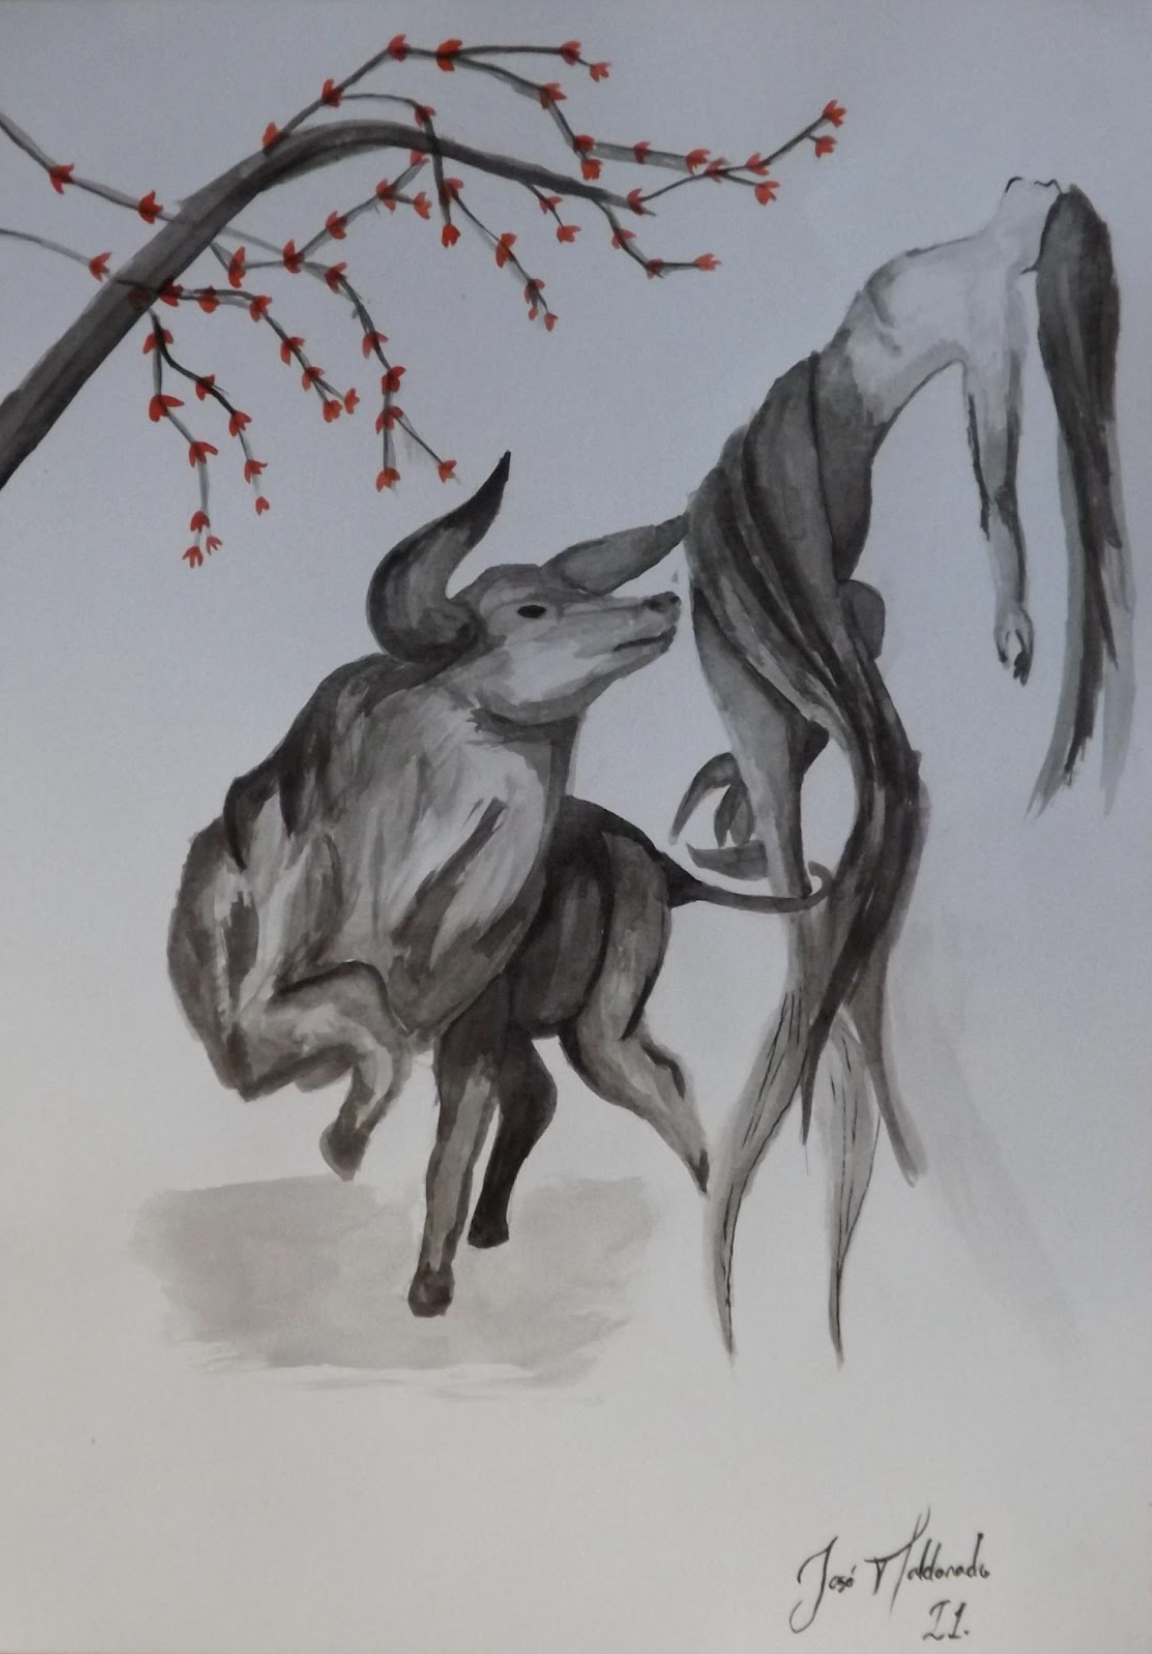
\includegraphics[width=1.0\textwidth]{verano en invierno.png}
\end{figure}
\clearpage

\poema{Corazón frío}
No hay que dejar que la soledad se encariñe con uno: nos vuelve blancos fáciles para la depresión que entra en silencio.

Cumplimos las reglas de siempre, aun sin estar de acuerdo. En el camino cruzamos a otros que también lo dieron todo y se quedaron sin nada.

Quizá por eso nos reconocemos: heridos que aprendieron a convivir con el frío.

Llegas con tu calor a invadir mi frío, pero hay un peligro en la costumbre.

Tengo el corazón frío no por falta de ganas, sino por miedo a acostumbrarme a tu calor y que después te vayas.

\poema{Incertidumbre}
Cuando un amor muere, otro nace, y allí estaba él; tenía cada cosa que podía enamorar a cualquiera.

Un amante que se mostró puro, único y atento me invitó a tomar su mano y llevarlo conmigo, temiendo aun así lo que podría pasar.

Descubrí que tras esa fachada se escondían cicatrices muy profundas, las cuales estuve dispuesto a ayudar a sanar.

Sus ojos ocultan un secreto que pesa, dejándolo sin paz alguna; su voz susurra una verdad oculta tras la mentira que rasga con penurias sus cuerdas vocales. Su corazón guarda un amor que aún no supera, alguien con quien quisiera volver, sabiendo así que no serviría de nada.

Es tiempo de tomar distancia, no por completo, sino de forma esporádica; aunque me duela, puede que sea la manera en que él se dé cuenta, o simplemente siga igual.

\poema{Tragedia en tres actos. Primer acto, Corazonada}
Intuición, ¿una maldición o una bendición? Sentí cómo aquella sombra oscura venía rompiendo cada uno de los hermosos recuerdos que existieron en el pasado.

Era inminente lo que estaba llegando: el faro que un día alumbró el camino a casa poco a poco fue apagando su luz.

Tus ojos ya no brillaban cuando mirabas mi rostro; ese brillo era ajeno a mi presencia. Ahora sé que encendieron su magia para aquel viejo ser que un día les dio vida.

No importa cuánto haya hecho o cuánto haya dado; lo que nunca perteneció a mí nunca pertenecerá en ningún momento.

\poema{Tragedia en tres actos. Segundo acto, Fractura}
Te di mi verdad y tú me diste lo oculto. Fue una caída libre, cual misil lanzado por un avión de guerra; caí al frío y duro suelo, pensando estúpidamente que lo haría entre tus brazos.

Mensajes de amor y lujuria leí en aquella pantalla. Fotos de dos pieles pecaminosas estrujaban mi sentir; aquel bello durmiente estaba retratado en su mirada.

Me siento tan avergonzado de haber sido un simple invitado en el juego de dos amantes.

Lo sabía… lo supe… la magia se estaba yendo y, con ella, mi sentir. Lo tuve entre mis manos y, como arena en el desierto, el viento lo disipó.

\poema{Tragedia en tres actos. Tercer acto, Reforma}
Al cargar con dolores del pasado entendí que solo terminaré haciéndome daño a mí mismo; el tiempo y la vida se encargarán de poner a cada uno en su respectivo lugar.

Duele mucho; sin embargo, con cada nuevo dolor que llega, una parte blanda de mí se va quedando más sólida.

Tantas mentiras, heridas, traiciones. No se lo deseo a nadie, pero si de algo estoy seguro es que siempre lo hice bien, en todos los aspectos, y ya con eso es suficiente para darme cuenta de que le dolerá más mi ausencia que la herida parchada en mi alma.

Aprendí que, para sobrevivir en este mundo, no debemos convertirnos en seres fríos o indiferentes; realmente debemos buscar la manera de ser más fuertes de corazón, sin perder la ternura del alma.

Tomaré toda esta tragedia y la convertiré en mi cura; que el amor propio me dé la sanación y cada error, una nueva oportunidad para alzar nuevamente mi vuelo.

\clearpage
\thispagestyle{empty}
\begin{figure}[h!]
    \centering
    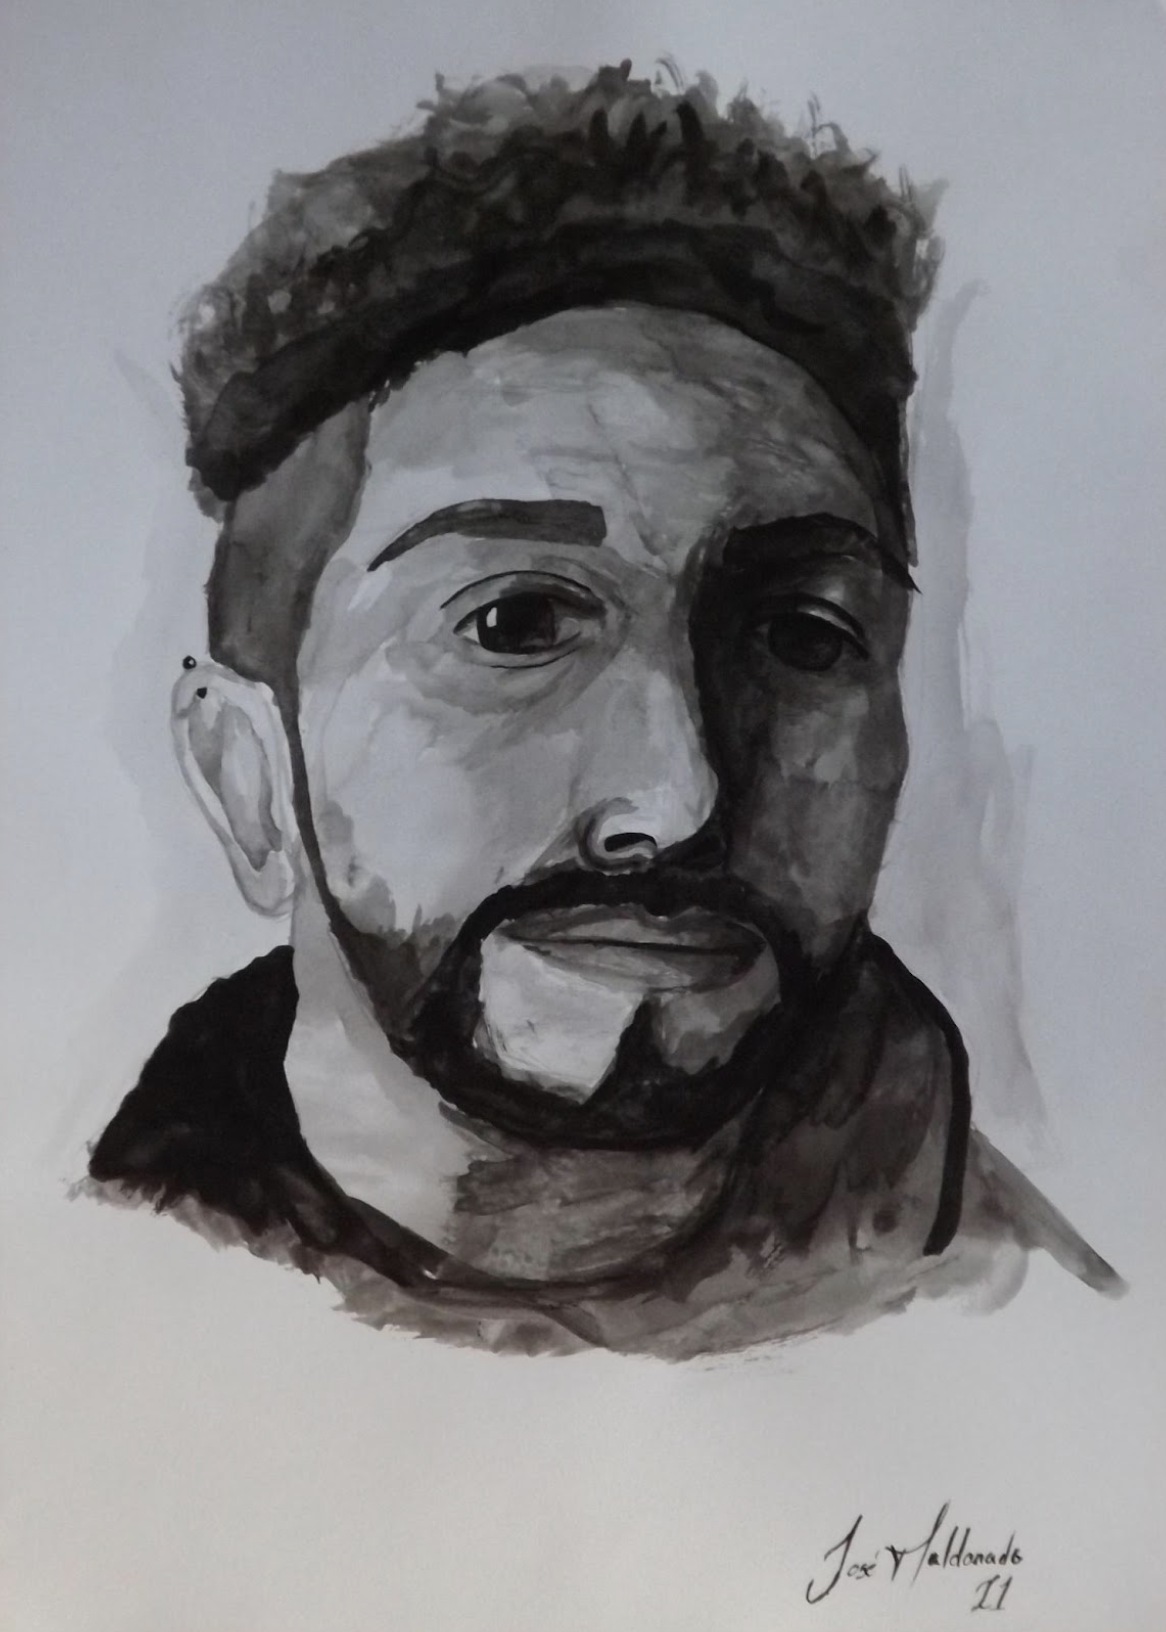
\includegraphics[width=1.0\textwidth]{tragedia.png}
\end{figure}
\clearpage

\poema{Apología del ser}
Hay personas que parecen una mentira, y hay otras que son mentiras deambulantes.

Procrastiné lo que realmente importaba para mí solo para entregarle mi tiempo a un reloj que necesitaba otro tipo de reparación.

Mientras me decías que estabas curando las heridas de tu sangre, en realidad remediabas las llagas del hostil.
Me viste sangrar y no te importó.

Imploré tu alquimia, esperé que transformaras mis heridas en algo que pudiera soportar, pero postergaste mi sanación.

—¿Por qué me mientes?

—¿Acaso no te di lo suficiente como para que vieras lo importante que eras para mí?

Y quizá ese fue mi error:

creer que entregarlo todo era suficiente para que alguien decidiera quedarse.

Aún recuerdo aquella noche en la que, entre lamentos y lágrimas, me dijiste que era demasiado para ti.

Debí haberte hecho caso.

Tú nunca fuiste suficiente para quedarte con todo lo que era.


\poema{2:15 am}
Estoy cansado.

Tengo el corazón en pedazos y el alma manchada. Me arrebataron sueños y metas que anhelaba cumplir algún día.

En mi lasitud, solo quiero descansar, poner el mundo en blanco y mirar de nuevo los ojos que vigilaron mis pasos desde pequeño.

Diría que la vida es injusta, pero sonaría como un niño caprichoso.

¿Está mal?

Ser racional es uno de mis fuertes. Puedo callar cada maldito pensamiento de ese pequeño destruido que únicamente quiere estar bien.

Cada lágrima que cae es un desperdicio. Cada nudo en la garganta es inservible. Cada sentimiento de tristeza, inútil.

Ser positivista es una excusa para creer que todo será mejor; ser negativista, otra para tirarse al abandono.
Y ser realista…

¿Realista?

Solo nos hace resignarnos a que algo va a acontecer, queramos o no.

Me acostaré en mi cama con el anhelo de que todo concluya.

Veré cómo voy a ser juzgado por personas que creen tener la respuesta a todo, y apoyado por quienes ya abrazaron la pérdida como si fuera su única realidad.


\poema{Viraha}
En intervalos de tiempo se refleja la bondad del ser humano; momentos tan efímeros que casi parecen invisibles.

Incrédulos son aquellos que desmoralizan la sinceridad de un amor decoroso para vivir aferrados al contradictorio espejismo que ofrece un corazón inhóspito.

Me condeno a la mentira que me vende la soledad, esa en la que no soy suficiente para mí mismo.

—¿Todo para qué?

Para saciar el hambre de los amantes corruptos y acribillar a los anhelantes de un amor nefelibato.

\poema{¡Oh! amado}
Ser sublime o subliminal, cada uno es dueño de su juicio y acreedor de su propio testimonio.

El ser indecoroso vacila ante el buen trato de quienes le admiran y el buen sentir de quienes le aman.

Toma el arma, aprieta el gatillo y dispara en lo más bajo de su víctima, dejándola inmóvil.

Por segunda vez, lo aprieta con fuerza y abre fuego directo en el corazón; un fuerte dolor estruja su pecho, arrebatándole casi todo su sentir.

No siendo suficiente, da el tiro final, justo en la cabeza, donde estallan las emociones y no se contienen las lágrimas…

Acabó con todo.

Entre el lúgubre cuerpo y el despiadado asesino solo queda el eco de las palabras que pusieron fin a lo que pudo haber sido un nuevo retoño de primavera en medio de la guerra.


\poema{Limbus}
Las pequeñas circunstancias cotidianas mi cabeza las manifiesta como una gran producción merecedora del prestigioso premio de la Academia.

Sueño a lo grande con tan solo un pequeño impulso, y con una pequeña idea hago revivir al más grande de los dioses y al más temido de los demonios.

Juega conmigo y haré que tu mente desconozca el momento en el que hizo un pacto de sangre contigo.

% ---------------------------------------------------------
% CAPÍTULO 2: ZEN
% ---------------------------------------------------------
\capituloconportada{ZEN}

\poema{Deliberación}
Entonces bajé por el sendero de rocas hasta llegar a la orilla del río y sumergí mis pies heridos.

Me adentré en sus aguas buscando lavar mis pecados.

El agua cubrió mi boca sin dejar escapar un murmullo.

Cerré los ojos y sentí cómo la corriente quería arrastrarme con ella.

Sin embargo, mis pies se aferraban aún más al suelo, sin importar cuán doloroso fuera.

Abrí los ojos y me vi frente a mi otro yo, una versión que guardaba mis más oscuros secretos.

Lo miré.

Él también me miró.

Ya no había hacia dónde huir.

Es hora de aceptar a mis demonios sin dejar que me dominen.


\poema{Lascivia}
Tan depravado como gallardo.

Caen las cadenas, el bajo suena más bajo, la inocencia se hace a un lado.

Una voz en mi interior susurra:

—¿Eres Afrodita Urania o Afrodita Pandemos?

Mi sudor es un licor embriagante.

La jauría está acechando; solo el macho alfa puede lamer mi piel de terciopelo.

¿Lo deseáis?

Columnas jónicas con ligeros roces en los fustes; un capitel capaz de cargar dos arcos cóncavos, admirados por arqueólogos sedientos de estudiarlos a fondo.

¿Estáis listo?

Mientras la marea sube y baja, la gravedad de la luna aumenta el oleaje; es estruendoso el sonido del agua entre las rocas.

Caigo por el precipicio hasta llegar a las suaves arenas de la playa.

Dulce elixir de la vida.


\clearpage
\thispagestyle{empty}
\begin{figure}[h!]
    \centering
    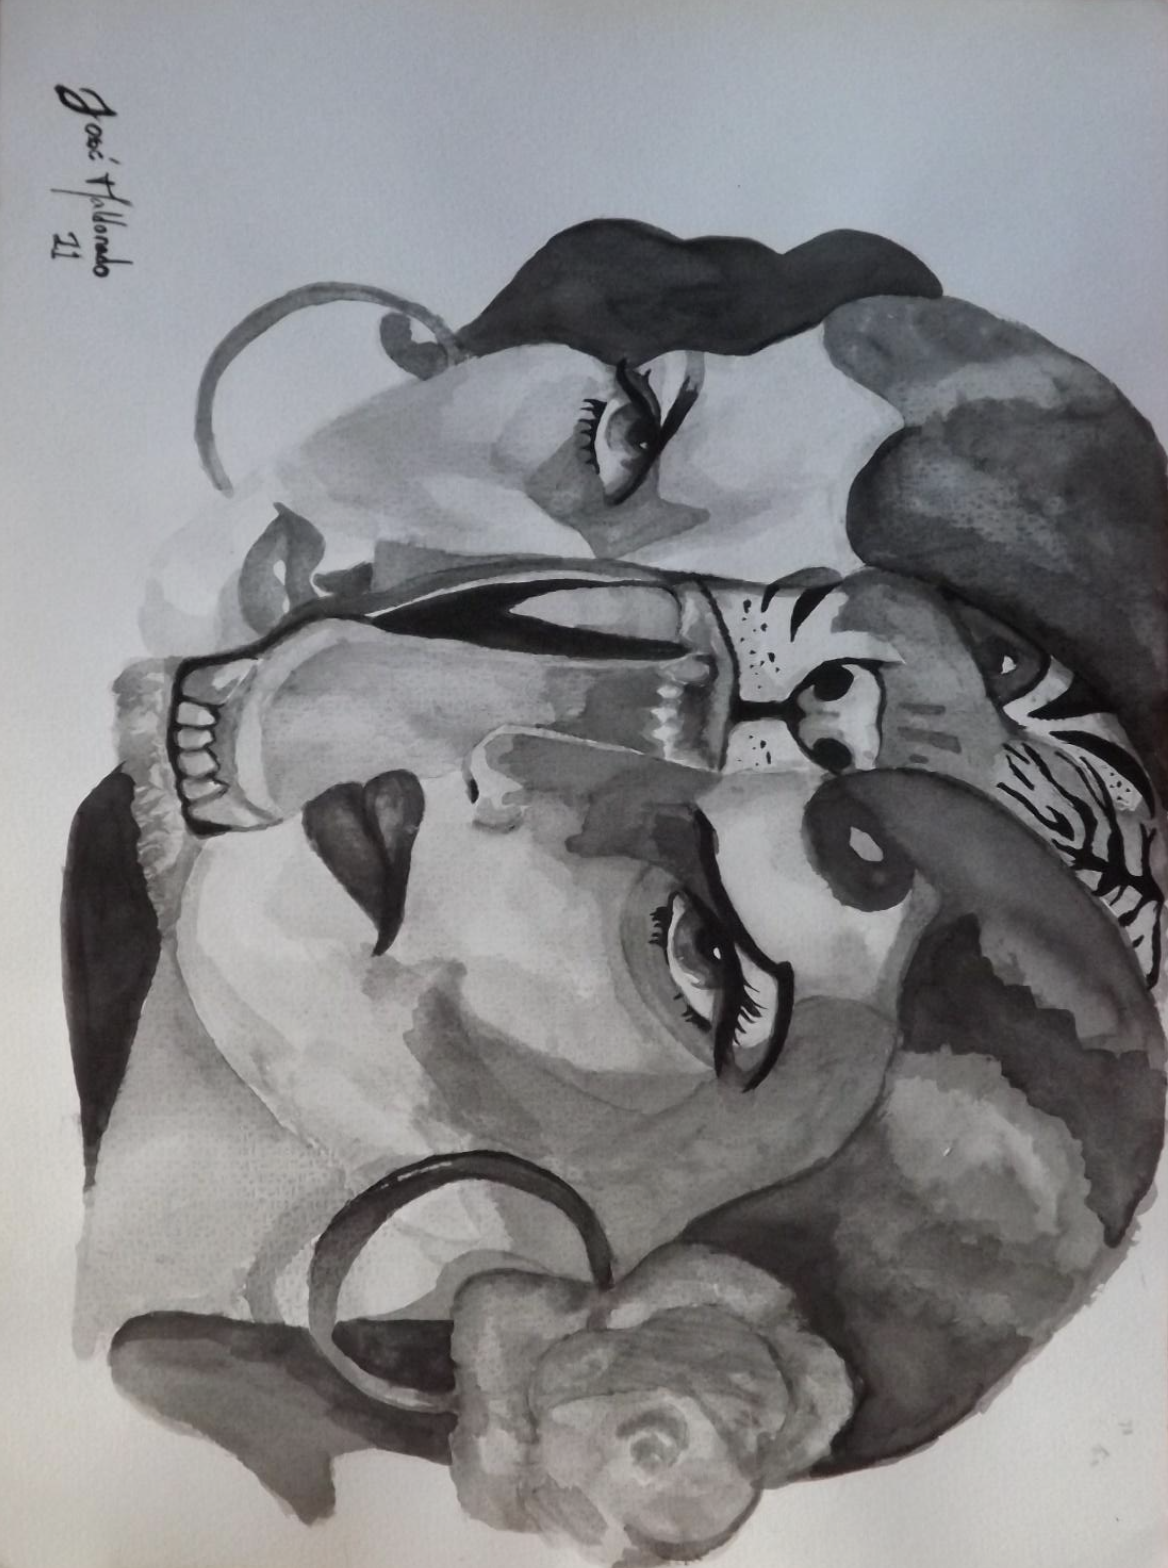
\includegraphics[width=1.0\textwidth]{lascivia.png}
\end{figure}
\clearpage

\poema{Redención}
Cuando entro en mi mente, nada puede destruirme.

Ellos odian mi ataraxia.

Camino sobre vidrio y fuego.

¿Qué hay adelante? ¿Felicidad efímera o tristeza limitada?

Las arenas del tiempo me tragan sin oponer resistencia.
Se abre la escotilla hacia un bucle de tiempo interminable.

Te ayudaré a salir de ahí.

Antes de irte, toma. Es para ti:

una parte de mi alma.

Sumérgela en tu santo grial y trágala.

Disfruta lo áspero o suave que se siente.

\clearpage
\thispagestyle{empty}
\begin{figure}[h!]
    \centering
    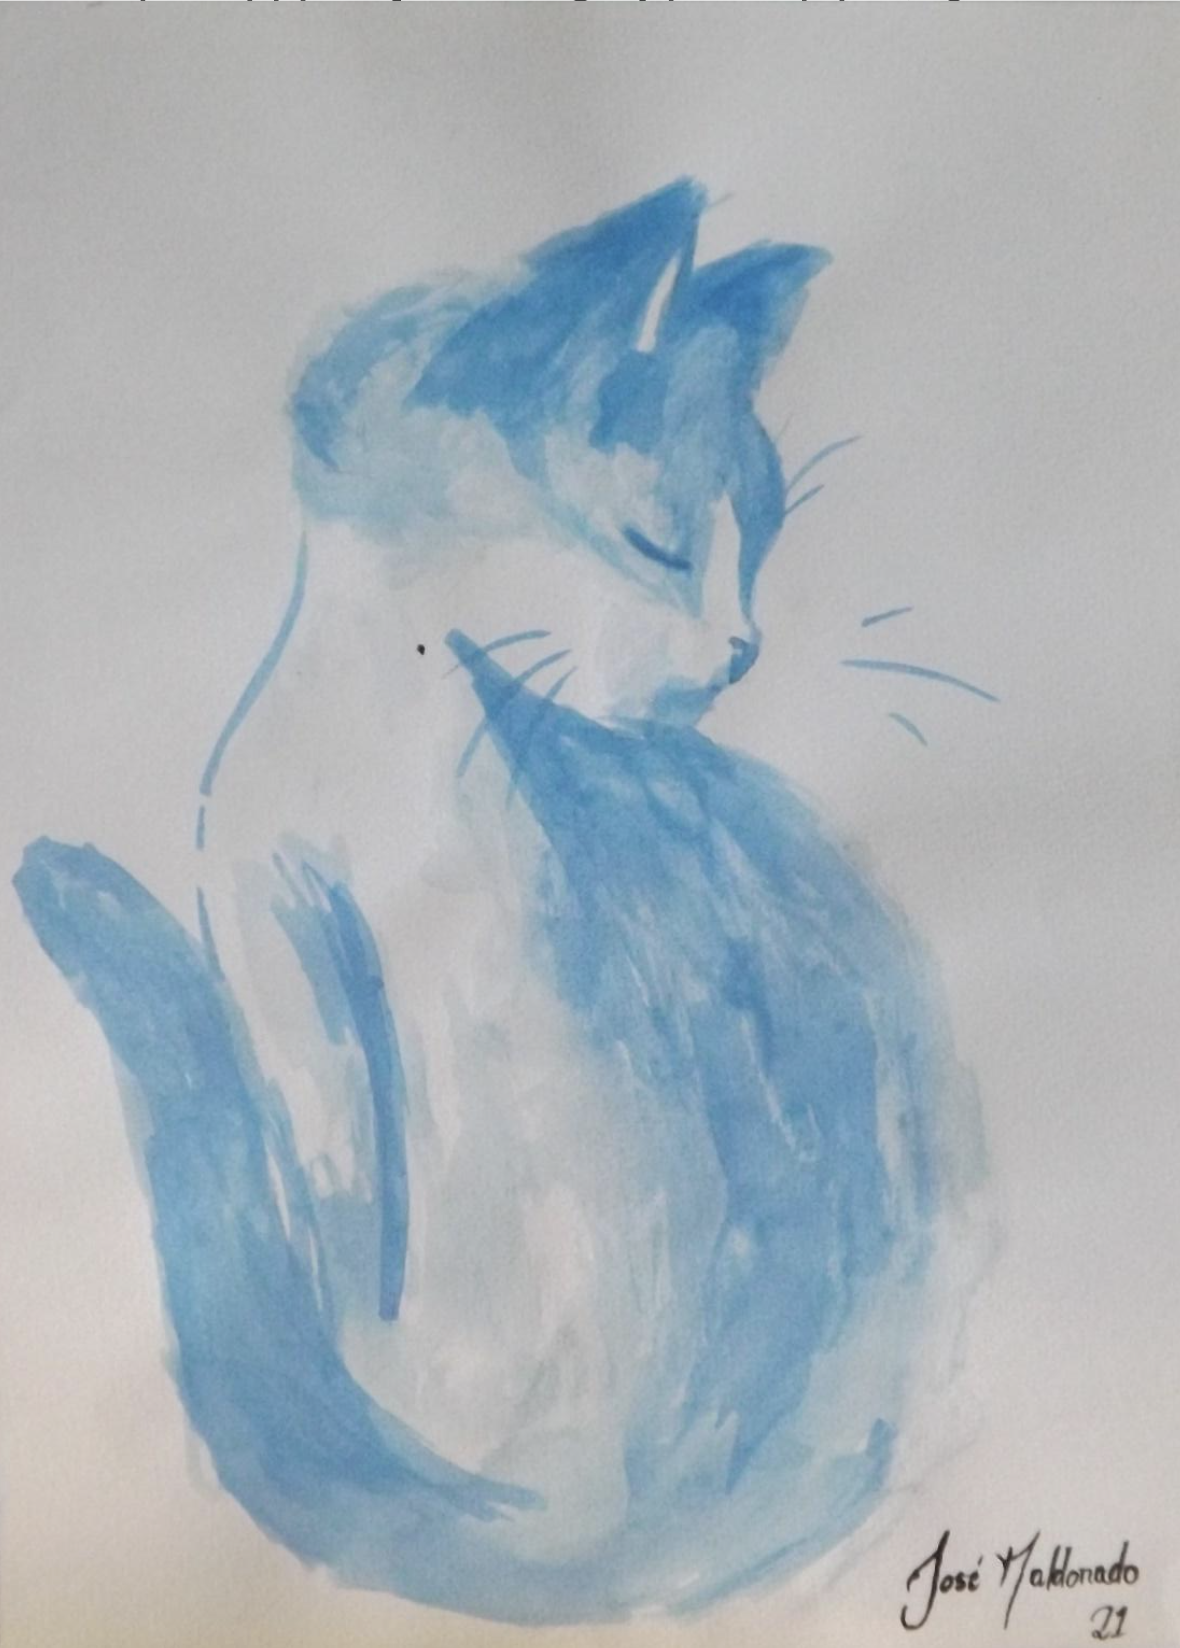
\includegraphics[width=1.0\textwidth]{redencion.png}
\end{figure}
\clearpage

\poema{Perdón}
Recogí de la orilla un trozo de leña arrojado por el mar y cavé hasta enterrarme a la mitad.

Viví años a la sombra de la vida, viendo cada disputa entre el sol y la luna por el dominio.

Mis piernas se entumecieron y pedí perdón a la arena por haberla invadido.

La brisa que traía consigo el oleaje se deslizaba dulcemente por mi rostro.

Mi espalda, quemada por el sol, gritaba de dolor, mientras mis manos acariciaban el tenue paso del tiempo.

¿Por qué?

¿Por qué me hago esto?

No lo merezco después de tantas batallas que rasgaron mi alma.

Miro al espejo y le veo llorar.

Ha sufrido mucho; sus cicatrices lo han marcado de por vida y, aun así, está de pie para dar más.

Perdón…

Lo siento por mí.

Algún día me perdonaré.

\poema{Responsabilidad}
Polvo eres y en polvo te convertirás.

Naciste del amor más puro que existe, un amor que, a pesar de la distancia, prevalecerá.

Soy hijo del león y de la victoria, engendrados en las tierras venezolanas, elevados sobre los cinco picos que brillan en mí cual aurora resplandeciente en el cielo.

Esta tierra, llena de misterios, te llevará por caminos verídicos y equívocos.

Depende de ti cuál tomar.

Solo te doy un consejo:

recuerda aquellas sabias palabras de tus ancestros.

Tal vez, entre ellas, encuentres las pistas que te indiquen cuál de esos caminos te llevará al éxito.


\poema{Equinoccio}
Y de nuevo, el mismo error:

adelantándome a cosas que no se pueden apresurar, dejándome llevar por un sentimiento lleno de fulgor que quema, pero que no puedo permitir que salga.

Debo dejar que me consuma hasta quedar en cenizas y renacer con el cuarto toque de la campana.

Esta vez es diferente.

Sentí alivio al escuchar un rechazo, como si mi alma necesitara sentir los pies sobre la tierra.

Entró como una bocanada de aire fresco.

Era la llave que necesitaba para cerrar esa puerta, esperando así que un tenue rayo de luz atravesara la cerradura y tocara el delicado y casi destruido brote de invierno.


\poema{Predilección de la nada}
Nunca me reprimo por mis sentimientos.

Soy un soñador ambulante que le sonríe a la misma tragedia sin importarme el precio que tenga que pagar.

Sabía que iba a doler.

Salí lastimado.

Sin embargo, pese a todo, no estoy en el fondo.

No estoy muerto.

Si duele es porque sigo vivo.

Y quizá sea precisamente ese dolor el que deba tomar para convertirlo en fuerza, para aprender de él y transformarme en una mejor versión de mí.

Pero…

¿ahora qué tengo?

¿La promesa de la resurrección, la certeza de que volveré a levantarme aunque algún día vuelva a caer?

¿O la catarsis para mi salvación, la oportunidad de aprender todo lo que este dolor puede enseñarme para trascenderlo y alcanzar una vida mejor?


\poema{Cafuné}
Reposé mi pulsera junto a su cama.

Tomé sus manos y las puse sobre mí.

Su cabello ondulado se enredaba con mi pendiente, tal como quería que se enredaran nuestras almas.

Sentado sobre él, solo miraba sus ojos castaños. Su piel morena era tan exótica como las playas brasileñas.

Su acento sensual provenía de la mezcla de varias naciones.

No podía evitar contornear con mis dedos el tatuaje de su pecho.

Somos como la luz y la oscuridad, el día y la noche: tan diferentes y, a la vez, tan similares.

Luz que ahuyentaba los demonios y oscuridad que cortaba a la mitad los deseos más profundos
.
Amantes de la vida o del interés.

En nuestros corazones habitan las intenciones más puras y más destructivas.

¿Somos capaces de armarnos el uno al otro, o de armarnos uno con las piezas del otro?


\poema{Mentoso}
Un vasto universo creado desde un lugar tan pequeño:
mi mente.

Mundos paralelos con posibilidades infinitas, donde un mismo acontecimiento puede tener distintas conclusiones.

Finales trágicos inventa mi mente para prepararme en caso de que ocurra lo peor.

Un escudo que me protege de frente, pero que no evita que me fracture desde el interior.

No sé si llamarlo prevención o destrucción:
torturarme poco a poco, imaginando una y otra vez la misma idea.

Creo que mañana me servirá para afrontar la maldita y cruda realidad.

Al final, puede que ya esté listo para lo peor.

De no ser así, que el remate me sorprenda y cure todas mis heridas, haciéndome más intangible a los demonios que en un principio creé.

\poema{Equilibrio}
Los cinco platos de la balanza a nivel debo tener.

Me obligo a llegar al final sin temer.

Es inevitable sentir temor cuando te fallaron en el amor.

“Un plato baja, cuatro suben”.

¡Qué fácil es ganar con un as y qué difícil es ganar la paz!

“Cae uno por un segundo mientras tres se mantienen flotando”.

Ganarle a la oscuridad de tu interior sin que se note el quiebre en el exterior.

“Ahora tres dominan el peso y dos están llenos del vacío”.
La recompensa llega con tanto sacrificio; la uso para mi beneficio y no puedo evitar culparme como un eterno maleficio.

“El último plato se balancea cual péndulo, sonando los pocos segundos antes de llegar a las doce”.

Así vas dando a los demás con el sentimiento más puro y tú solo te escarmientas, persiguiendo con apuros un futuro que realmente es inseguro.

“El equilibrio está completo”.

Todos los puntos distribuidos, pero la balanza quedó en la misma posición inicial.

Con peso en sus cinco platos, hace un gran esfuerzo mecánico para mantener la misma estabilidad que tenía sin cargar ninguno.


\poema{Aquiles}
Somos sombras cobijadas bajo el intermitente parpadear de los faros en las avenidas.

Ocho jugadores. Se abren las apuestas.

Veintisiete, cuarenta y cinco, cincuenta y cuatro, sesenta y cuatro, diecinueve, treinta y seis.

Las mesas generan expectativas tan inciertas que hacen que la envidia se esconda detrás del generoso y el avaro se vea majestuoso.

La hora veinticinco se hace eterna tras atender con paciencia y generosidad a aquellos cuyas túnicas verdes adornan el salón principal.

\poema{alfa y omega}
Entre catorce lápidas esculpidas existe la verdad de una vida simulada perfecta.

Mentiras escuálidas gritadas a los vientos revelan un sinfín de caras que ayer parecían reales.

Tragedia, tragedia, tragedia…

La respuesta a ese mísero sentimiento solo existe en el nudo que creaste en tu lengua.

Procuras un cambio pragmático, tan subyacente que ni tú mismo eres capaz de llevarlo a cabo, por miedo a ser rechazado entre los falsos acreedores de la verdad absoluta.

Ve a la fuente sin desearlo.

Tal vez así encuentres la respuesta a aquello que no andabas buscando.

\clearpage
\thispagestyle{empty}
\begin{figure}[h!]
    \centering
    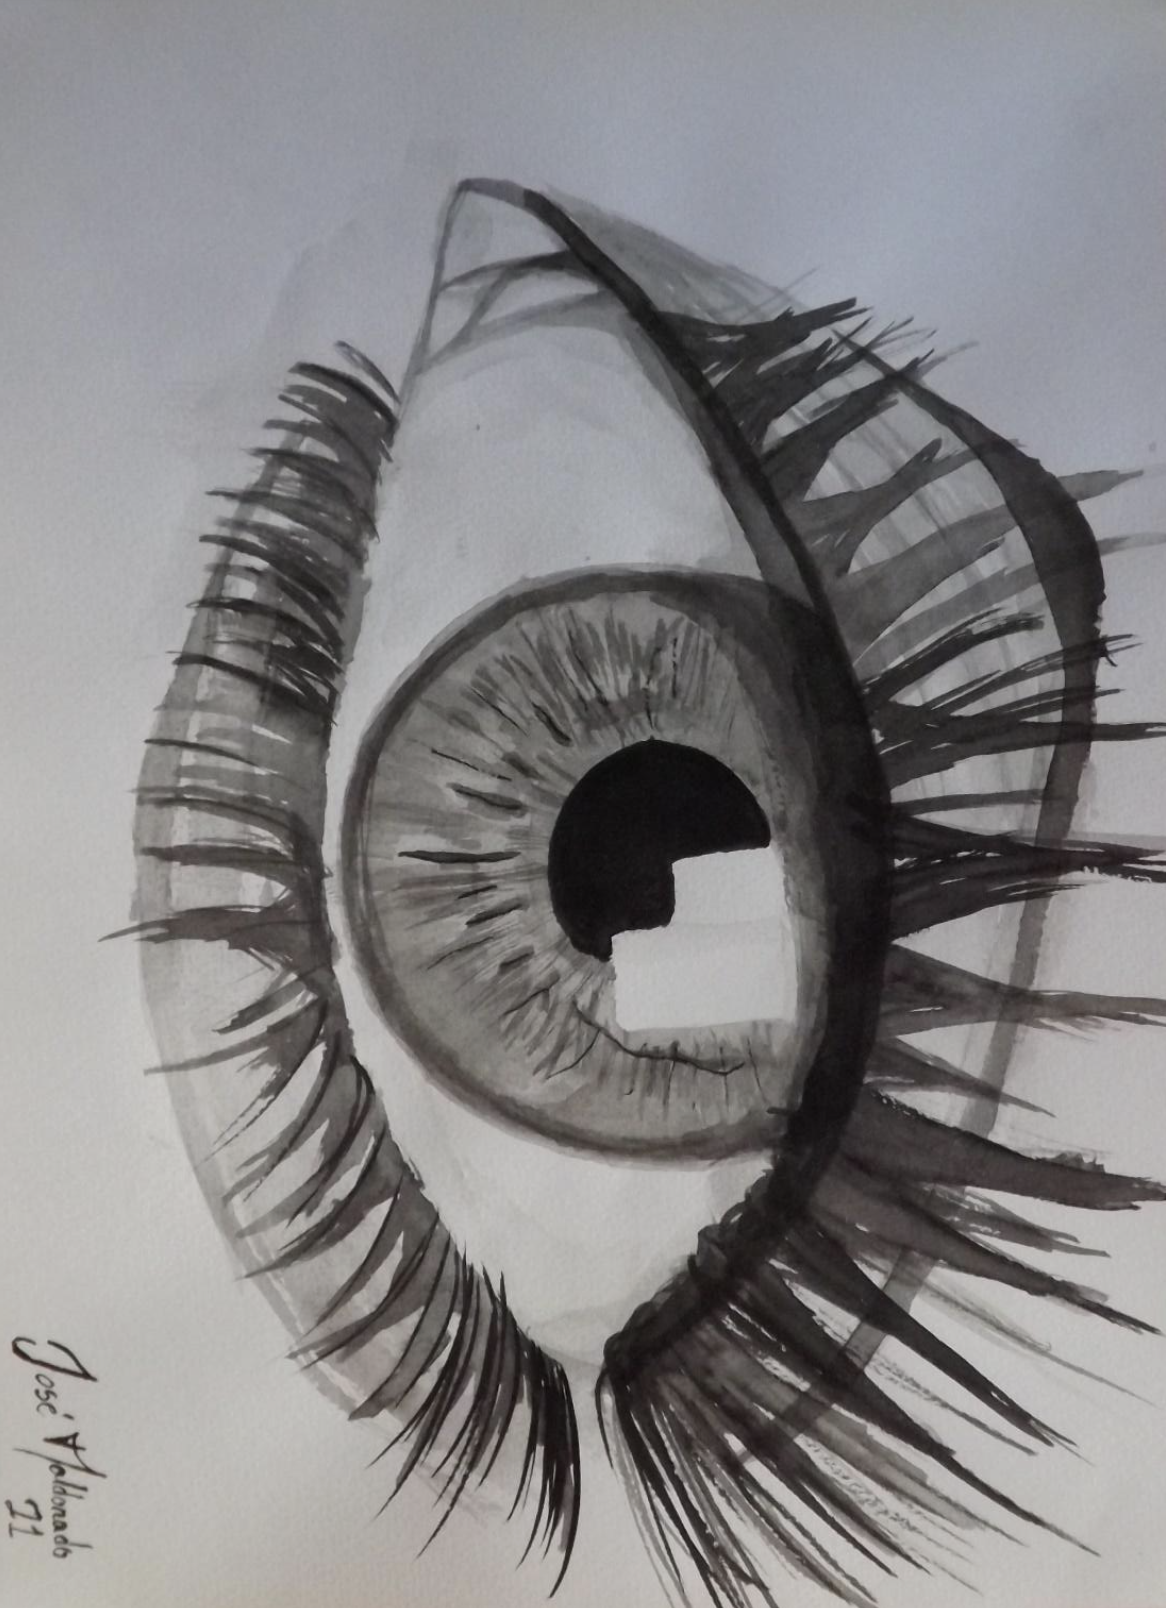
\includegraphics[width=1.0\textwidth]{alfayomega.png}
\end{figure}
\clearpage

\poema{Bilita mpash}
En mi cuarta resurrección anduve descalzo en el laberinto del Minotauro.

Por largo tiempo atravesé el interminable camino hasta encontrarme con la Parca.

Ya estaba muerto:

una criatura tan mala e inocente a la vez.
Vi a la bestia sin vida tendida en el suelo.

Pisé la sangre que estaba derramada y pensé:

¿Por qué maldicen el destino de un ser cuyas acciones no tienen nada que ver con el pecado de los dioses?

Mi espíritu lloraba sin encontrar consuelo en tanta incertidumbre.

Me hinqué, sequé las lágrimas del indefenso animal, arranqué un trozo de mi túnica y cubrí su destruida mirada.

Me acosté junto a él, esperando que lo que quedaba de nosotros desapareciera entre el vasto pastizal.


% ---------------------------------------------------------
% CAPÍTULO 3: ÉTER
% ---------------------------------------------------------
\capituloconportada{ÉTER}

\poema{Resurrección}
Pensé que volvería a caer:

partidas, problemas, discusiones, dudas, una tras otra, sin darme un respiro.

Es como si rompiera una pared con mis manos, anhelando salir, pero encontrando otra aún más resistente del otro lado.

Puertas y ventanas cerradas.

Un pequeño rayo de luz corta a la mitad la espesa oscuridad y apunta a mi pecho.

Mientras más me acerco, más crece aquel cálido resplandor.

Pese a todo, el fénix sigue resucitando de entre las cenizas, cada vez más consciente de su justiprecio.

Los rostros son cada vez más notables, el denuedo más sólido y la verdad más clara que la trápala.

\clearpage
\thispagestyle{empty}
\begin{figure}[h!]
    \centering
    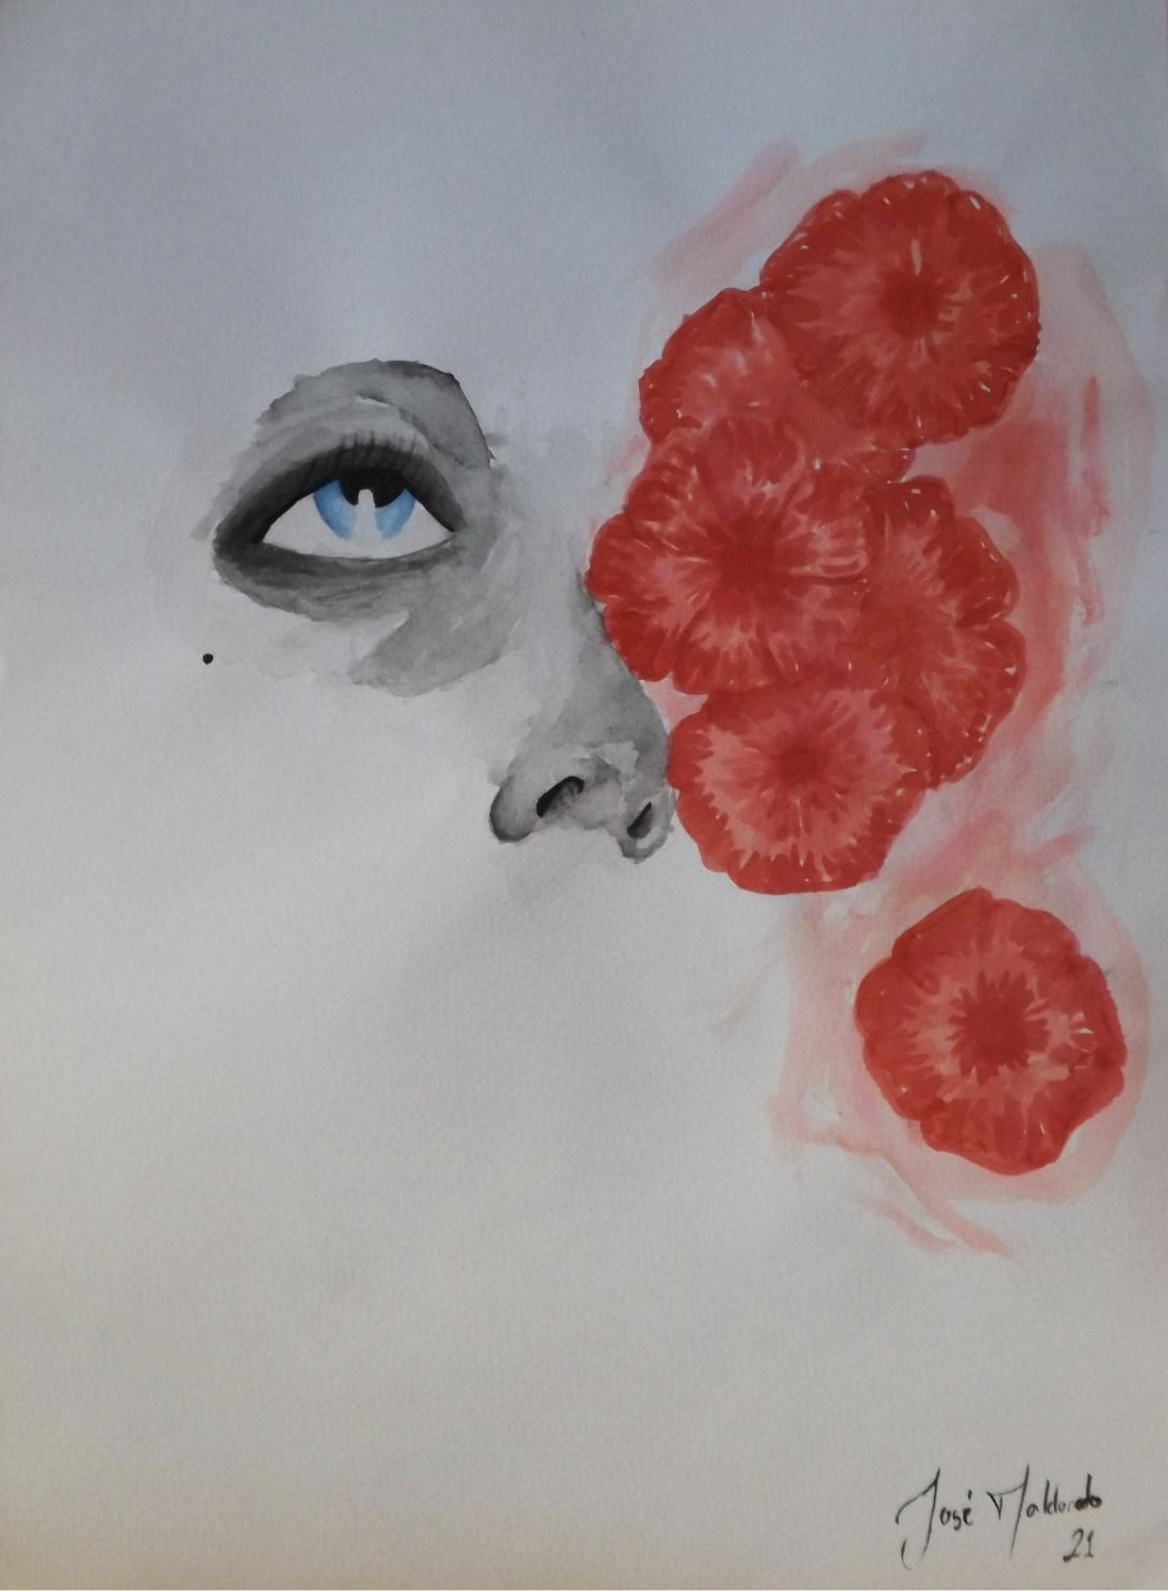
\includegraphics[width=1.0\textwidth]{resurreccion.png}
\end{figure}
\clearpage

\poema{Ecuanimidad}
Tomé por sentado que todo iba a seguir bien.

Mientras más fuerte soplaba el huracán, más me aferraba a mis sólidas bases, bases que construí con el dominio de los catorce titanes que se doblegaron ante mí.

Un bolígrafo, un pincel, un tintero y un papel se convirtieron en mis armas.

Escribí el rostro y pinté las palabras de mis miedos hasta transformarlas en lo que ahora son mis soportes.

Ya sé que mientras en el mañana se disipen las cenizas, recogeré los temores del ayer y haré que ardan hoy en la perpetua llama del tiempo.

\poema{Muerte del letargo}
Dormí en la divina calma.

Estuve inmerso durante tres días seguidos, sin ayuno ni arrepentimiento, hasta que el reloj marcó las tres y treinta.

Desperté sin fuerzas para levantarme. No podía pensar con claridad ni hablar.

Aun así, continué.

Poco a poco me puse de pie y con cada paso que daba podía dominar el siguiente.

Fui ascendiendo a la cima con las manos atadas a la espalda y los ojos vendados.

Temeroso de lo que podía pasar, sojuzgué las tres etapas del camino.

Descansé siendo el primero en la puerta del alfa y el omega.

Descendí los nueve círculos como lo hizo Alighieri:

muerto en vida y lleno de tantas penurias, rogaba llegar a las nueve esferas del Paraíso para así ver a Dios.

Sin embargo, antes de escalar las siete laderas del Purgatorio, debía beber del Lete y de Eunoé para así poner fin a esta comedia.


\poema{Limerencia}
Fue perfecto, un momento etéreo, pero sublime a la vez.

El roce de nuestras bocas entonaba una sinfonía placentera que inspiraba a las mismas musas.

Mientras tu piel sudorosa palpaba lo más profundo de mi ser, yo sentía el inminente final acercándose, después de horas en las que solo quería que aquel momento fuera eterno.

Te vas, dejando una promesa tan vacía como tus intenciones carnales.

Sin embargo, no olvidarás aquellas noches taciturnas en las que anhelabas con deseo entrar en el paraíso prohibido.

¿Me extrañas a mí o al fantasma que pecaminosamente recorría cada rincón de tu áspera, pero deleitable, piel?

\poema{Extranjeros}
Rojo carmesí.

Las noches largas a la orilla del río. Luces reflejadas en lo más profundo de sus ojos, casi tan cautivadoras como el reverberar de los faroles sobre el tenue oleaje.

Sus ojos eran los de un asesino que miraba con deseo al trozo de carne que, aún en vida, añoraba encontrar un poco de humanidad en aquellos dos amantes del narcisismo.

La pulsera que un día reposé al lado de su cama ya no volverá a mí, así como no volverá lo único real que un día pudiste tener.

Un amante de invierno que una noche caminó tomado de mi mano se desvaneció cual efímero movimiento de la hermosa bailarina que proclamaba su libertad.

Es notorio que mi pluma y papel ya no lloran la partida de quienes creía tan reales.

Sin darme cuenta, resultaron ser dos falsos actores que arrastraban consigo su mal teatro, cual almas en pena cargando con sus pecados.

\poema{Renacimiento}
Un vaso que solía estar a tope un día quedó casi vacío.

Intentó tomar el agua de otras fuentes, pero ninguna le correspondía; y, si había alguna parecida, no era capaz de ser compartida.

Estar casi vacío le hizo sentir que la única manera de subsistir era que otro le compartiera de su contenido.

Un vaso decidió compartir con él su dulce brebaje.

Muy en el fondo, sabía que no iba a ser para siempre; aun así, decidió hacerlo suyo.

Fue tan perfecto que no se percató de que el dolor venía silenciosamente cubriéndolo todo.

Pasado el tiempo, el líquido desapareció.
Suplicó por más.

Sin embargo, al darse cuenta de que ya era el final, sucumbió ante la pena y la tristeza.

Hundido en la miseria, alzó la mirada
y vio a su sexto yo:

la versión más antigua de él, aquella que había aprendido que si no buscas la salvación por ti mismo, no la vas a encontrar en nadie más.

Ahora, de sus penurias, creará su propia fuente:
la fuente de la vida.

Una fuente que no se agotará estando solo ni acompañado; una que pueda compartir con el vaso que aprecie su dulce verdad.


\poema{Cartas al vacío}
He pasado por amores fugaces, aquellos que en pocos días se ganaron su puesto;

otros que recitaron poesía con sus palabras, envolviendo a este ser con frases llenas de inteligencia;

unos que se burlaron de cada buena acción que hice por ellos; y otro que valió cada año, siendo aquel al que le debo gran parte de lo que me he convertido.

El amor es poderoso siempre y cuando realmente exista.
Puede cambiar personas, cosas, ideales, creencias e incluso al mundo.

Amarse a sí mismo es la clave para dar amor.

Cuando aprendemos a apreciar las pequeñas cosas de la vida, los grandes detalles dejan de parecer tan grandes.
Puede haber más amor en una flor recogida del pavimento que en un rosal lleno de espinas.

\poema{Origen}
De entre grandes lomas y peñascos se cuela el frío abrazador que nos representa.

Blanca nieve se desliza por los enormes picos que se asoman en casi todo su terreno y adornan aquellos monumentos que simbolizan mi tierra natal.

Abundante folclore corre por mi pueblo como sangre por mis venas.

De lo criollo no me safo: 

nací en sus brazos, caminé sobre sus pies, dormí en su regazo y crecí bajo su mirada.

Así es: de ahí soy y de ahí seré, esté donde esté.
Aunque la historia te arranque algún día del mundo, tu esencia prevalecerá por siempre.

\clearpage
\thispagestyle{empty}
\begin{figure}[h!]
    \centering
    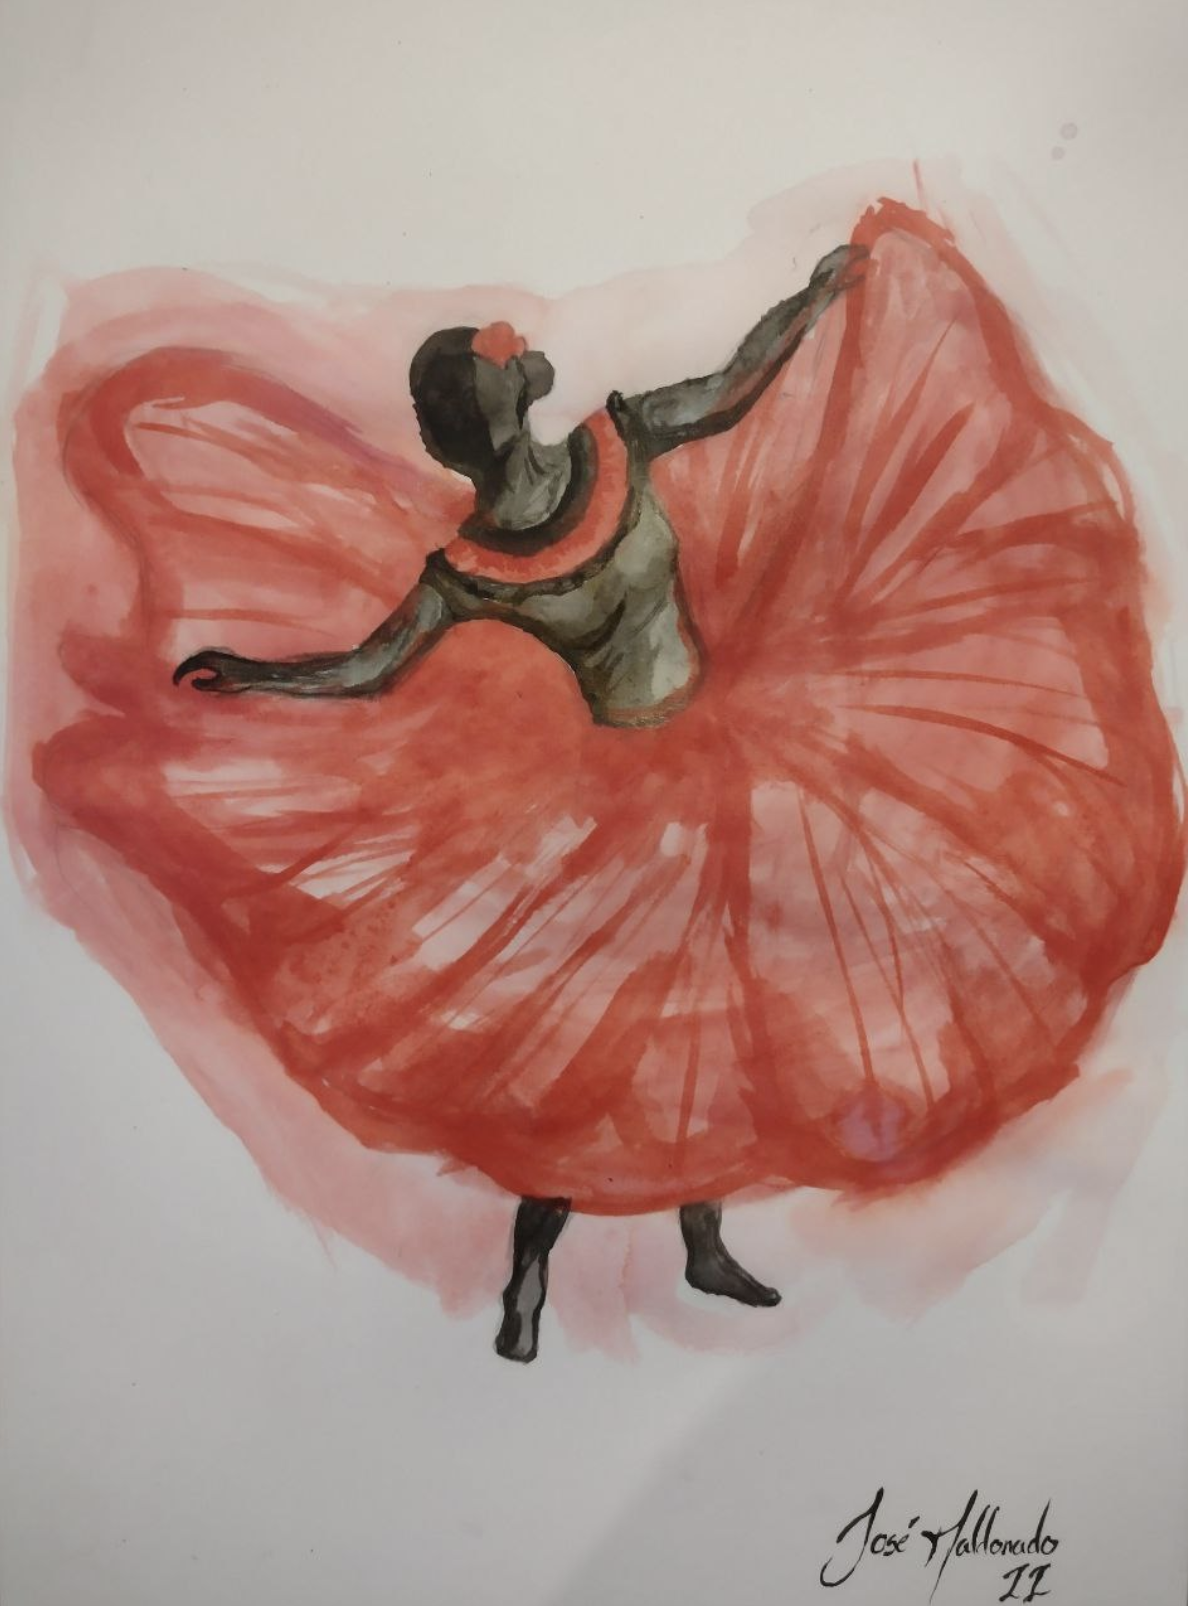
\includegraphics[width=1.0\textwidth]{origen.png}
\end{figure}
\clearpage

\poema{Amnistía}
Perdono al tiempo por llevarse todas mis sonrisas.

Perdono a la vida por robarme buenos momentos.

Perdono al destino que me fue impuesto, trayendo consigo un sinfín de martirios.

Perdono al amor que me hizo pasar por alto una infidelidad.

Perdono al extraño que un día me prometió la luna y terminó por hacerme creer un lunático.

Me perdono a mí por no darme lo que realmente merezco.

\poema{Alejandro}
Un guerrero.
Cualquier apodo queda corto cuando has sufrido el rechazo, el odio y el desprecio.

Consiguió en sí mismo la valentía para seguir en un mundo que le había dado la espalda.

Tomó cada palabra que venía de la inmundicia y las convirtió en alas para sobrevolar a aquellos que no conocían su verdadero yo.

No es meritado por todo, pero tampoco desmerecedor de nada.

Sin embargo, su esfuerzo le ha permitido ganarse el amor de quienes ven su verdadero ser.

Es enemigo del rey y aliado del pueblo;
difamado por su sangre, vive bajo el apoyo de los aprovechados.

Pase lo que pase, su amor será real y sublime.
Quienes un día le apuñalaron por la espalda, mañana le rogarán auxilio.

Y aquellos que ayer fueron recíprocos, brindarán y cantarán con él al unísono de la abeja reina.

\clearpage
\thispagestyle{empty}
\begin{figure}[h!]
    \centering
    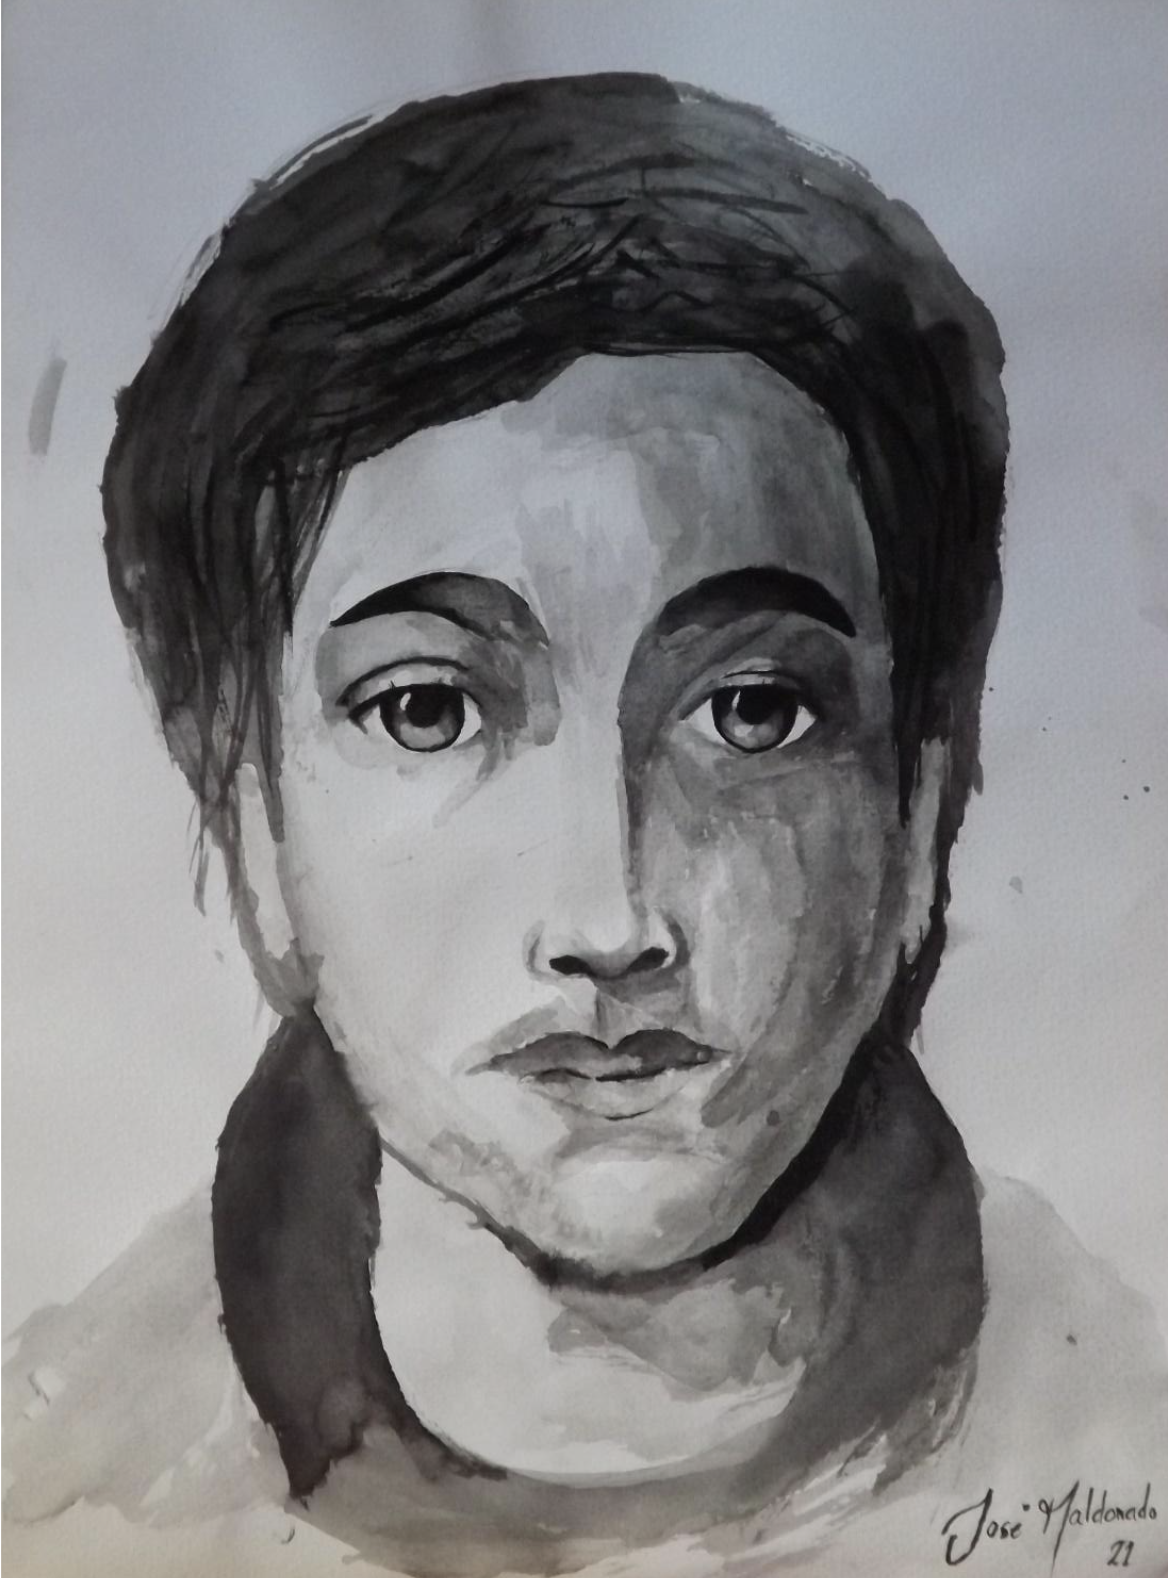
\includegraphics[width=1.0\textwidth]{alejandro.png}
\end{figure}
\clearpage

\poema{Ascenso}
Está bien sentirse mal en momentos de quiebre.

Cuando no puedo seguir de pie, reestructuro todos mis pensamientos con el fin de encontrar otro punto focal.

Puedo cambiar el sentido de mi angustioso pesar; sin embargo, en ocasiones respeto el mal querer de mi melancolía.

Cuando esta quiere marcharse, se retira pacíficamente, dando paso a la tranquilidad.

Con todas estas circunstancias, veo que la mejor manera de lidiar con nuestros destructores es entender que no siempre están para hacernos mal.

En ocasiones, nos alertan de que una etapa está por terminar y una nueva comienza.


\poema{Nunchi}
Soy chapado a la antigua.

Aún sueño, cual poeta, con recibir un amor recíproco; uno que no sea adivino, pero que pueda apreciar las necesidades más simples de alguien que ama el detallismo y la atención.

No pido que modifiques las normas ya regidas, como lo hizo el rey Enrique XIII,
ni que construyas un palacio como lo pidió Shah Jahan.

Con simple sinceridad basta.

\poema{Pérfido}
No estoy aquí para ser el entretenimiento de nadie.

Por más que me guste alegrar corazones, me enrabia el hecho de que existan egoístas que rompen las esperanzas de los filántropos.

Te ríes de las desgracias de los pobres y desgracias la vida del inocente.

Falsa tu sonrisa. Mentirosas tus promesas.

Caminas sobre los cadáveres de tus seguidores con tal de salvar tu pellejo.

“Divide y vencerás”…

Así ganaste.

No la guerra; ganaste el odio de quienes confiaron en ti y descubrieron tus artimañas.

Aplaudo tu teatro lleno de falsedades.

Estoy impaciente por ver cuánto dura el tiempo que el destino te dio para tocar una estrella y no una simple bombilla de luz.

\poema{Meraki}
Hay artistas que viven para vender su talento, y hay otros que lucran con inspirar a los demás.

Era enero en ese entonces.

Lo que debería ser un buen comienzo de año se había convertido en el inicio de la peor etapa de lo que hasta ahora llevaba de vida.

Ingenuamente, pensé que era el comienzo.

No lo era.

Era el desarrollo de un oscuro pesar que doblegó todo mi ser.

En mi inexistencia, un lápiz me escribió.

Entre tanto desconsuelo, escuché el álbum que encendió la chispa que un día se había apagado.

Como un limón me sentí: ácido por dentro, pero hermoso por fuera.

Transmuté toda esa mierda hasta que se convirtió en amor; amor propio que hace surgir a cualquiera que esté dispuesto a continuar vivo.

Canté mis versos a quienes querían escucharme,
y allí escuché lo que me cambiaría por el resto de mi vida:

—Me inspiraste.



% ---------------------------------------------------------
% GLOSARIO
% ---------------------------------------------------------
\clearpage
\chapter*{Glosario}
\vspace{-0.5em}
{\color{black}\rule{\textwidth}{0.4pt}} \par \vspace{0.8em}
\addcontentsline{toc}{chapter}{Glosario}

\begin{description}
    \item[\textbf{Afrodita Pandemos:}] Manifestación de la diosa Afrodita que representa el amor terrenal, físico, carnal y las pasiones vulgares o populares.
    \item[\textbf{Afrodita Urania:}] Manifestación de la diosa Afrodita que representa el amor celestial, puro, espiritual y platónico.
    \item[\textbf{Alighieri (Dante Alighieri):}] Poeta italiano autor de la \textit{Divina Comedia}, obra estructural dividida en Infierno (nueve círculos), Purgatorio (siete laderas) y Paraíso (nueve esferas celestiales).
    \item[\textbf{Ataraxia:}] Estado de tranquilidad, serenidad e imperturbabilidad del alma en el que no existen temores ni deseos ansiosos.
    \item[\textbf{Bangover:}] Es un juego de palabras en inglés que significa (resaca sexual), mezcla: \textit{Bang:} coloquialmente, tener sexo / un encuentro sexual y \textit{Hangover:} resaca.
    \item[\textbf{Bilita mpash:}] Expresión de origen bantú que describe un sueño increíble, hermoso y profundamente placentero (lo opuesto a una pesadilla).
    \item[\textbf{Cafuné:}] Palabra en portugués que describe el acto de pasar cariñosa y suavemente los dedos por el cabello de la persona amada.
    \item[\textbf{Conticinio:}] Hora de la noche en que todo está en silencio y los seres vivos descansan.
    \item[\textbf{Denuedo:}] Valor, intrepidez, esfuerzo y brío al afrontar situaciones difíciles.
    \item[\textbf{Emancipación:}] Liberación respecto de una autoridad, de una tutela o de cualquier condición de dependencia o sometimiento.
    \item[\textbf{Enrique XIII:}] Referencia lírica/aliterada a las reformas históricas de las normas monárquicas relativas al matrimonio y las leyes reales.
    \item[\textbf{Eunoé:}] Según la tradición dantesca, río del Purgatorio que restituye la memoria de las buenas acciones pasadas tras haber bebido del Lete.
    \item[\textbf{Filántropo:}] Persona que se distingue por su amor hacia sus semejantes y por sus obras en bien de la comunidad.
    \item[\textbf{Inhóspito:}] Lugar o espacio incómodo, agresivo, deshabitado o hostil donde resulta difícil habitar.
    \item[\textbf{Justiprecio:}] Valoración o tasación justa, exacta y ponderada de una cosa o cualidad.
    \item[\textbf{Lasitud:}] Estado de cansancio, debilidad, fatiga física o desfallecimiento del espíritu.
    \item[\textbf{Lete:}] En la mitología griega y dantesca, el río del olvido del Inframundo cuya agua borra el recuerdo de las culpas y los pecados pasados.
    \item[\textbf{Lid:}] Combate, pelea, disputa o contienda violenta entre dos partes.
    \item[\textbf{Limerencia:}] Estado mental involuntario en el que una persona experimenta una obsesión amorosa e intensa necesidad de reciprocidad afectiva.
    \item[\textbf{Melindrosa:}] Que demuestra un escrúpulo, finura, afectación o delicadeza excesiva y exagerada.
    \item[\textbf{Meraki:}] Palabra griega que significa hacer algo con alma, creatividad, pasión o amor; dejar una huella de uno mismo en lo que se realiza.
    \item[\textbf{Nefelibata:}] Dicho de una persona soñadora, que anda por las nubes y no se apercibe de la realidad objetiva.
    \item[\textbf{Nunchi:}] Concepto coreano que define la habilidad sutil de percibir e interpretar los estados de ánimo, sentimientos y necesidades no expresadas de los demás.
    \item[\textbf{Pérfido:}] Persona desleal, infiel, traidora o que falta a la fe empeñada.
    \item[\textbf{Pragmático:}] Enfoque o actitud que prioriza la práctica, la utilidad y los hechos concretos sobre la teoría o lo ideal.
    \item[\textbf{Quimera:}] Monstruo mitológico; también se refiere a una ilusión, fantasma o creación imaginaria que se da por real.
    \item[\textbf{Shah Jahan:}] Emperador mogol que mandó a construir el Taj Mahal como monumento al amor eterno tras la muerte de su esposa Mumtaz Mahal.
    \item[\textbf{Sojuzgué (Sojuzgar):}] Dominar, someter, sujetar o poner bajo el control propio por la fuerza o la determinación.
    \item[\textbf{Taciturna:}] Persona callada, silenciosa, propensa a la melancolía o a la tristeza en sus pensamientos.
    \item[\textbf{Trápala:}] Engaño, alboroto, falsedad o enredo con el que se pretende confundir a alguien.
    \item[\textbf{Viraha:}] Término en sánscrito que describe el sufrimiento, vacío y consciencia del amor causados por la separación o distancia de la persona amada.
\end{description}

\end{document}
